\chapter{The Resonance Search on the Dimuon Signature}
\label{chapter:dimuon}

\section{Introduction}

Owing to its unprecedented high energy, the Run 1 and early Run 2 of ATLAS has long focused on the high mass resonances searches that was not accessible to any other previous experiments. This approach has left the relatively low mass resonances that are competitive in sensitivity unexplored. In the resonance search that decays into two leptons in particular, the resonance mass region above Z boson peak has been searched for since the beginning of Run 1. However, the mass region below the Z mass peak remains uncovered to this date. Novel particles with an LHC scale observable coupling is predicted by many models, some of them are related to the dark matter models explored in Chapter~\ref{chapter:DM}.

\begin{figure}[!htb]
    \begin{center}
        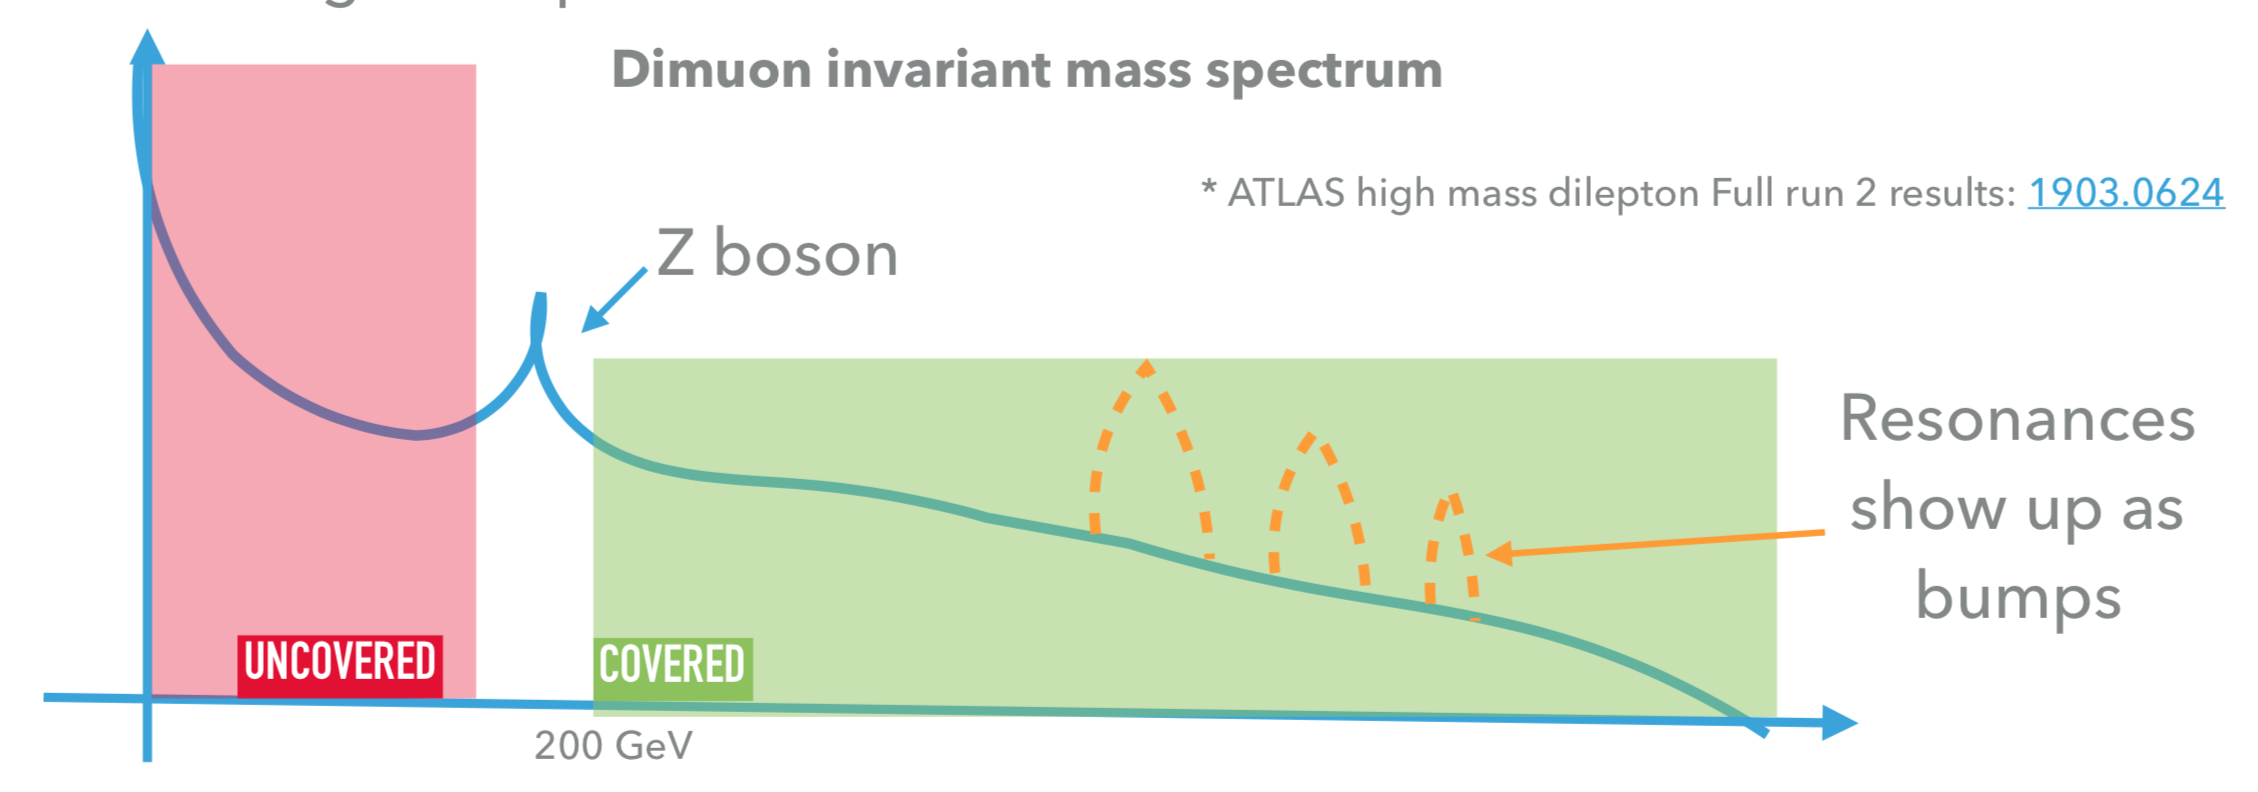
\includegraphics[width=0.75\textwidth]{figures/chapter_dimuon/dimuonStudies}        
        \caption{
        This cartoon illstrate the target signal region of the analysis and how it has not been covered by the previous high-mass dilepton analysis. }
            \label{fig:dimuonstudies}
    \end{center}
\end{figure}
\FloatBarrier
   
This study share many similar motivations as the analysis presented in Chapter~\ref{chapter:dijetISR}, where the dark matter mediator $Z^\prime$ is projected to decay into two jets. In this analysis, the $Z^\prime$ couples instead to leptons. Since ATLAS collide partons, there are fewer background on leptons than jet processes, this allows lower transverse momentum lepton events to be saved. Using two muons as the resonance final state items, even lower mass resonances can be searched for this study would
explore dark matter related resonances down to 4 GeV. To avoid the quarkonium background between 4-10 GeV and the Z boson in 80 GeV, this analysis searches for resonances in the 10-68 GeV range.

This chapter presents an on-going analysis conducted in ATLAS. The data preparation, trigger chain, event and object calibration that is completed and validated for the analysis is presented in Section~\ref{}. The full statistical strategies, which is currently that utilizes Gaussian Process as the background estimation method is covered in Section~\ref{}. All strategies are in place and ready for the analysis to be unblinded. The analysis utilizes data using proton--proton collision in ATLAS
recorded at a center-of-mass energy of $\sqrt{s}=$ 13 ~\TeV up to 139 $fb^{-1}$ of integrated luminosity. The projected result is interesting to the theoretical community for the dark matter mediator reinterpretation as well as its statement possible for many other models, which include W$\prime$, quantum blackholes and axions. The result of this study is complementary to the dilepton search done here with its exploration of a lower mass resonance region, and have is projected to have limits to
the CMS~\cite{CMS-PAS-EXO-19-018} and LHCb~\cite{Aaij:2722971} results published.

\section{The Search Channels}
In ATLAS, not all collision events are stored due to the limitation in processing bandwidth. Triggering is the processing and storage of selective events, more details are described in Chapter~\ref{chapter:ATLAS}. Triggering requires physical cuts in the event objects, sometimes this introduces features in the data that is not predicted in the physics. An example is the muon $P_{T}$ requirement in triggering produces a trigger turn-on curve seen in the inclusive histogram in Figure~\ref{fig:turnon}.
Non-physical feature in background can lead to difficulty in background modelling. In view of this, two different search channels are employed for the analysis for maximal sensitivity. In the 40-68 GeV region, the inclusive dimuon signal as shown in ~\ref{fig:dimuonFeynman} is searched for. In the 10-40 GeV of the analysis, a boosted ISR signal as shown in ~\ref{fig:dimuonISRFeynmann} is used for the analysis. They are the region highlighted in blue in Figure~\ref{fig:turnon}.In the boosted channel, an additional cut of dimuon $P_{T}>14 GeV$ is applied to both the signal and the background. This cut produces a smooth background and retains a signal efficiency of >90\%. This strategy is effective in producing a background that can be modelled and maximizing sensitivity. 
This two channel treatment is based on a pheno-study first done in this paper\cite{2014}. Changes has been made to accomodate the increase in the center-of-mass energy of the analysis. 

\begin{figure}[!htb]
    \begin{center}
        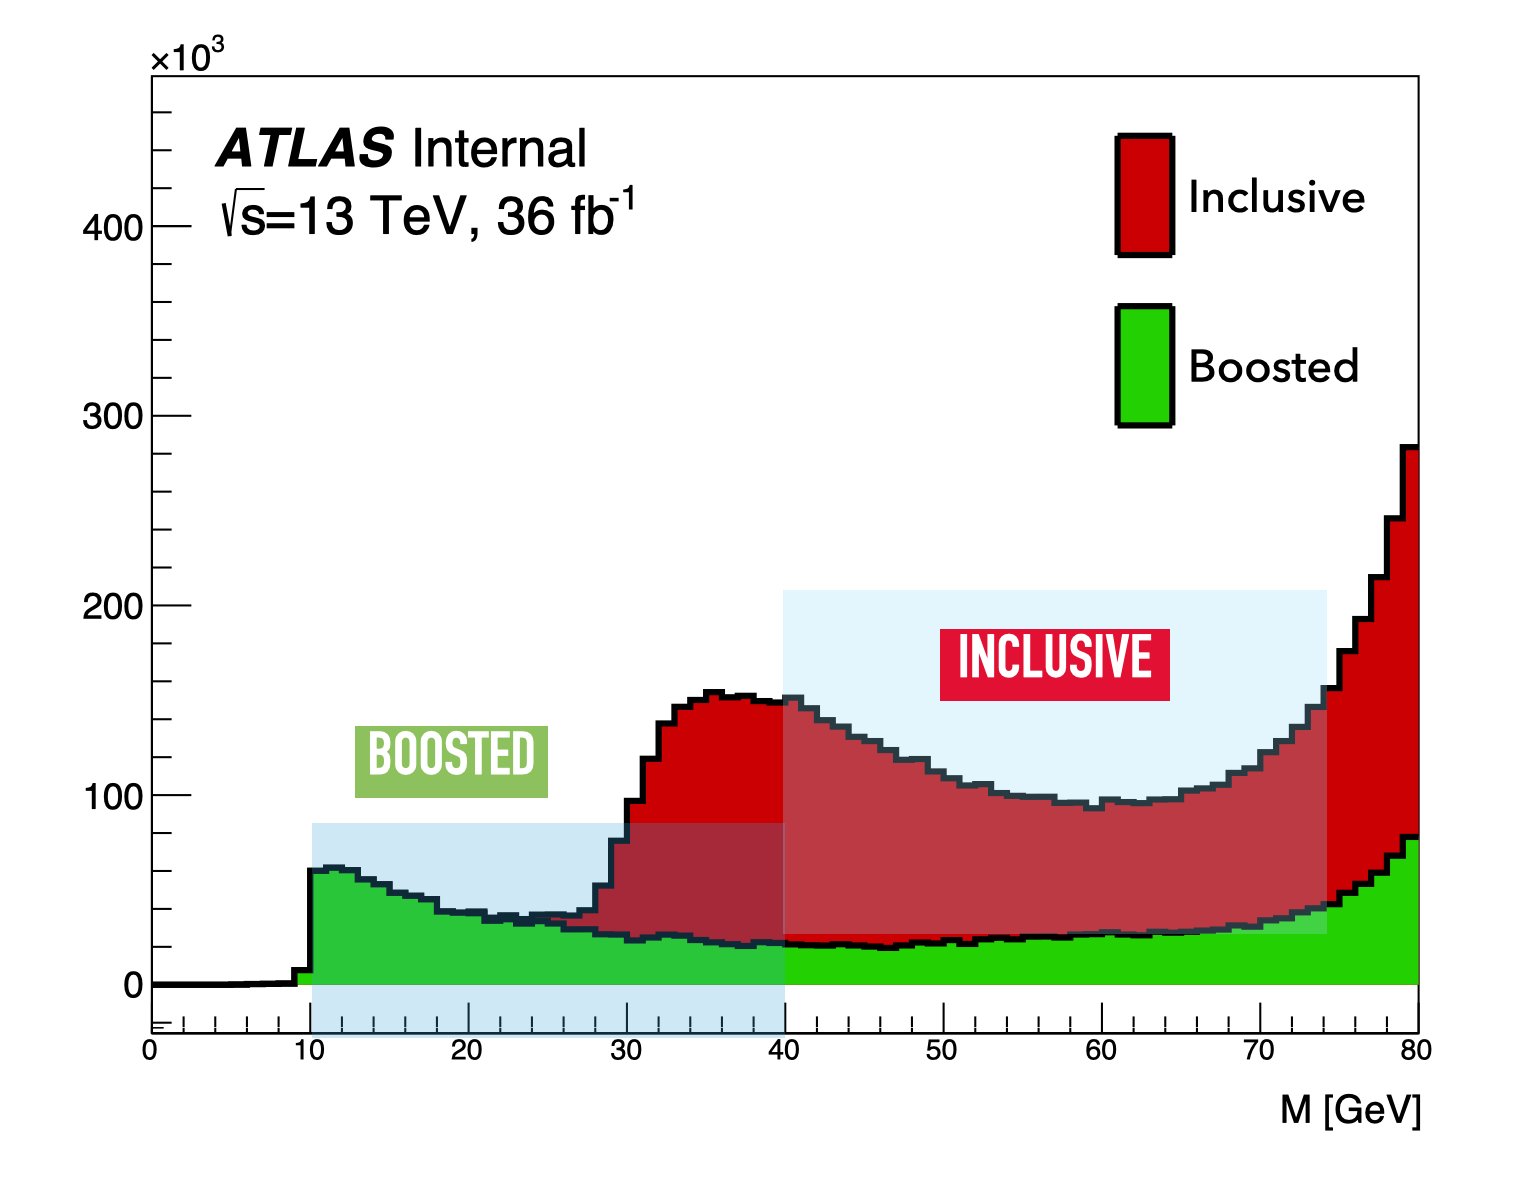
\includegraphics[width=0.75\textwidth]{figures/chapter_dimuon/turnon}
        \caption{
        This figure shows the trigger turn on curve in the inclusive dimuon channel at 40 GeV(Red) . Utilizing a minimal dimuon $P_{T}$ cut in the boosted channel made it possible to recover a smooth background in the lower mass region from 10-45 GeV(Green). Samples used here are MC16a ATLAS full simulation listed in section~\ref{table:MC}.
        }
        \label{fig:turnon}
    \end{center}
\end{figure}
\FloatBarrier

\section{Signal Theoretical Model}
The analysis uses the dark matter LHC benchmark model and dark photon model outlined in Section~\ref{sec:LHCDM} of Chapter~\ref{chapter:DM}.
Other models that are of interest and can be reinterpreted for this analysis includes the W\', the quantum blackholes,and axion models. Limit setting on generic Gaussian shape of various width will enable ease for reintepreation with tools like RECAST.
Figure~\ref{fig:dimuonFeynman} and Figure~\ref{fig:dimuonISRFeynmann} show the Feynmann diagram of the signal used for the analysis 
The signal are generated through ATLAS full simulation: the tree level event is generated through Madgraph5\_aMC@NLO~\cite{}; the parton showering is simulated through Pythia8~\cite{} and detector effect is added on through Geant4~\cite{}. More details on MC generation of ATLAS can be found in Chapter~\ref{chapter:common_analysis_items}.

\begin{figure}[!htb]
    \begin{center}
        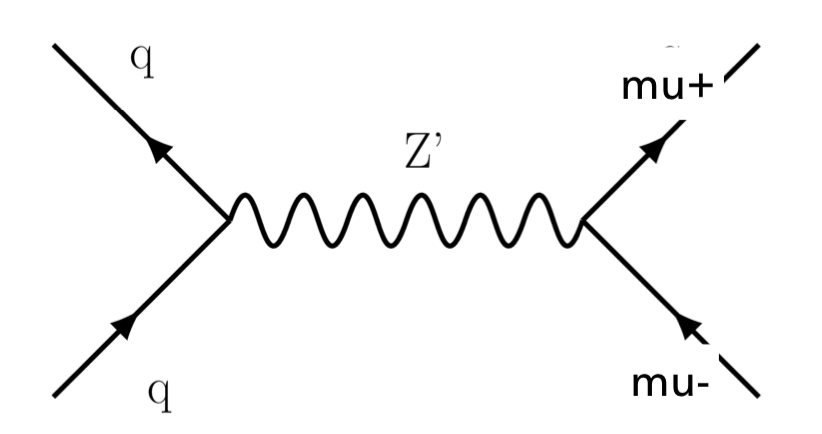
\includegraphics[width=0.45\textwidth]{figures/chapter_dimuon/dimuonFeynman}
        \caption{
            This figure shows the Feynmann diagram of the inclusive dimuon signal as the signal for the analysis. 
        }
    \label{fig:dimuonFeynmann}
    \end{center}
\end{figure}
\FloatBarrier

\begin{figure}[!htb]
    \begin{center}
        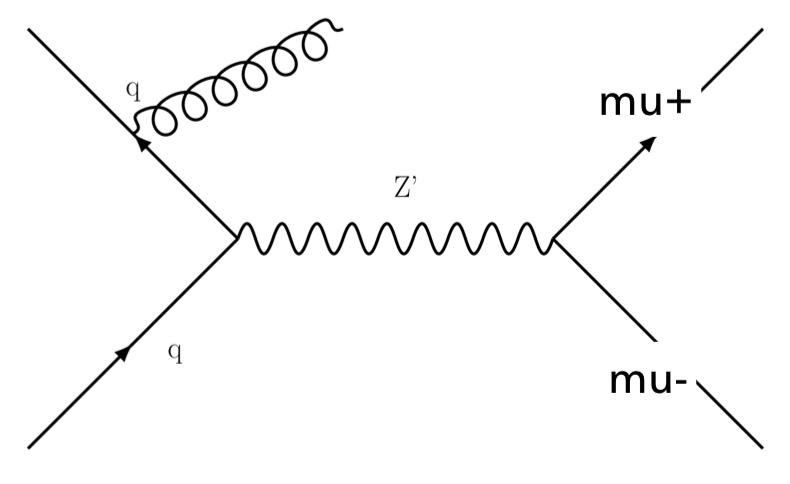
\includegraphics[width=0.45\textwidth]{figures/chapter_dimuon/dimuonISRFeynmann}
        \caption{
        This figure shows the Feynmann diagram of the boosted dimuon ISR signa used as the signal for the analysis. }
            \label{fig:dimuonISRFeynmann}
    \end{center}
\end{figure}
\FloatBarrier

    %Details on the signal generation from the jira ticket

%\begin{figure}[!htb]
%    \begin{center}
%        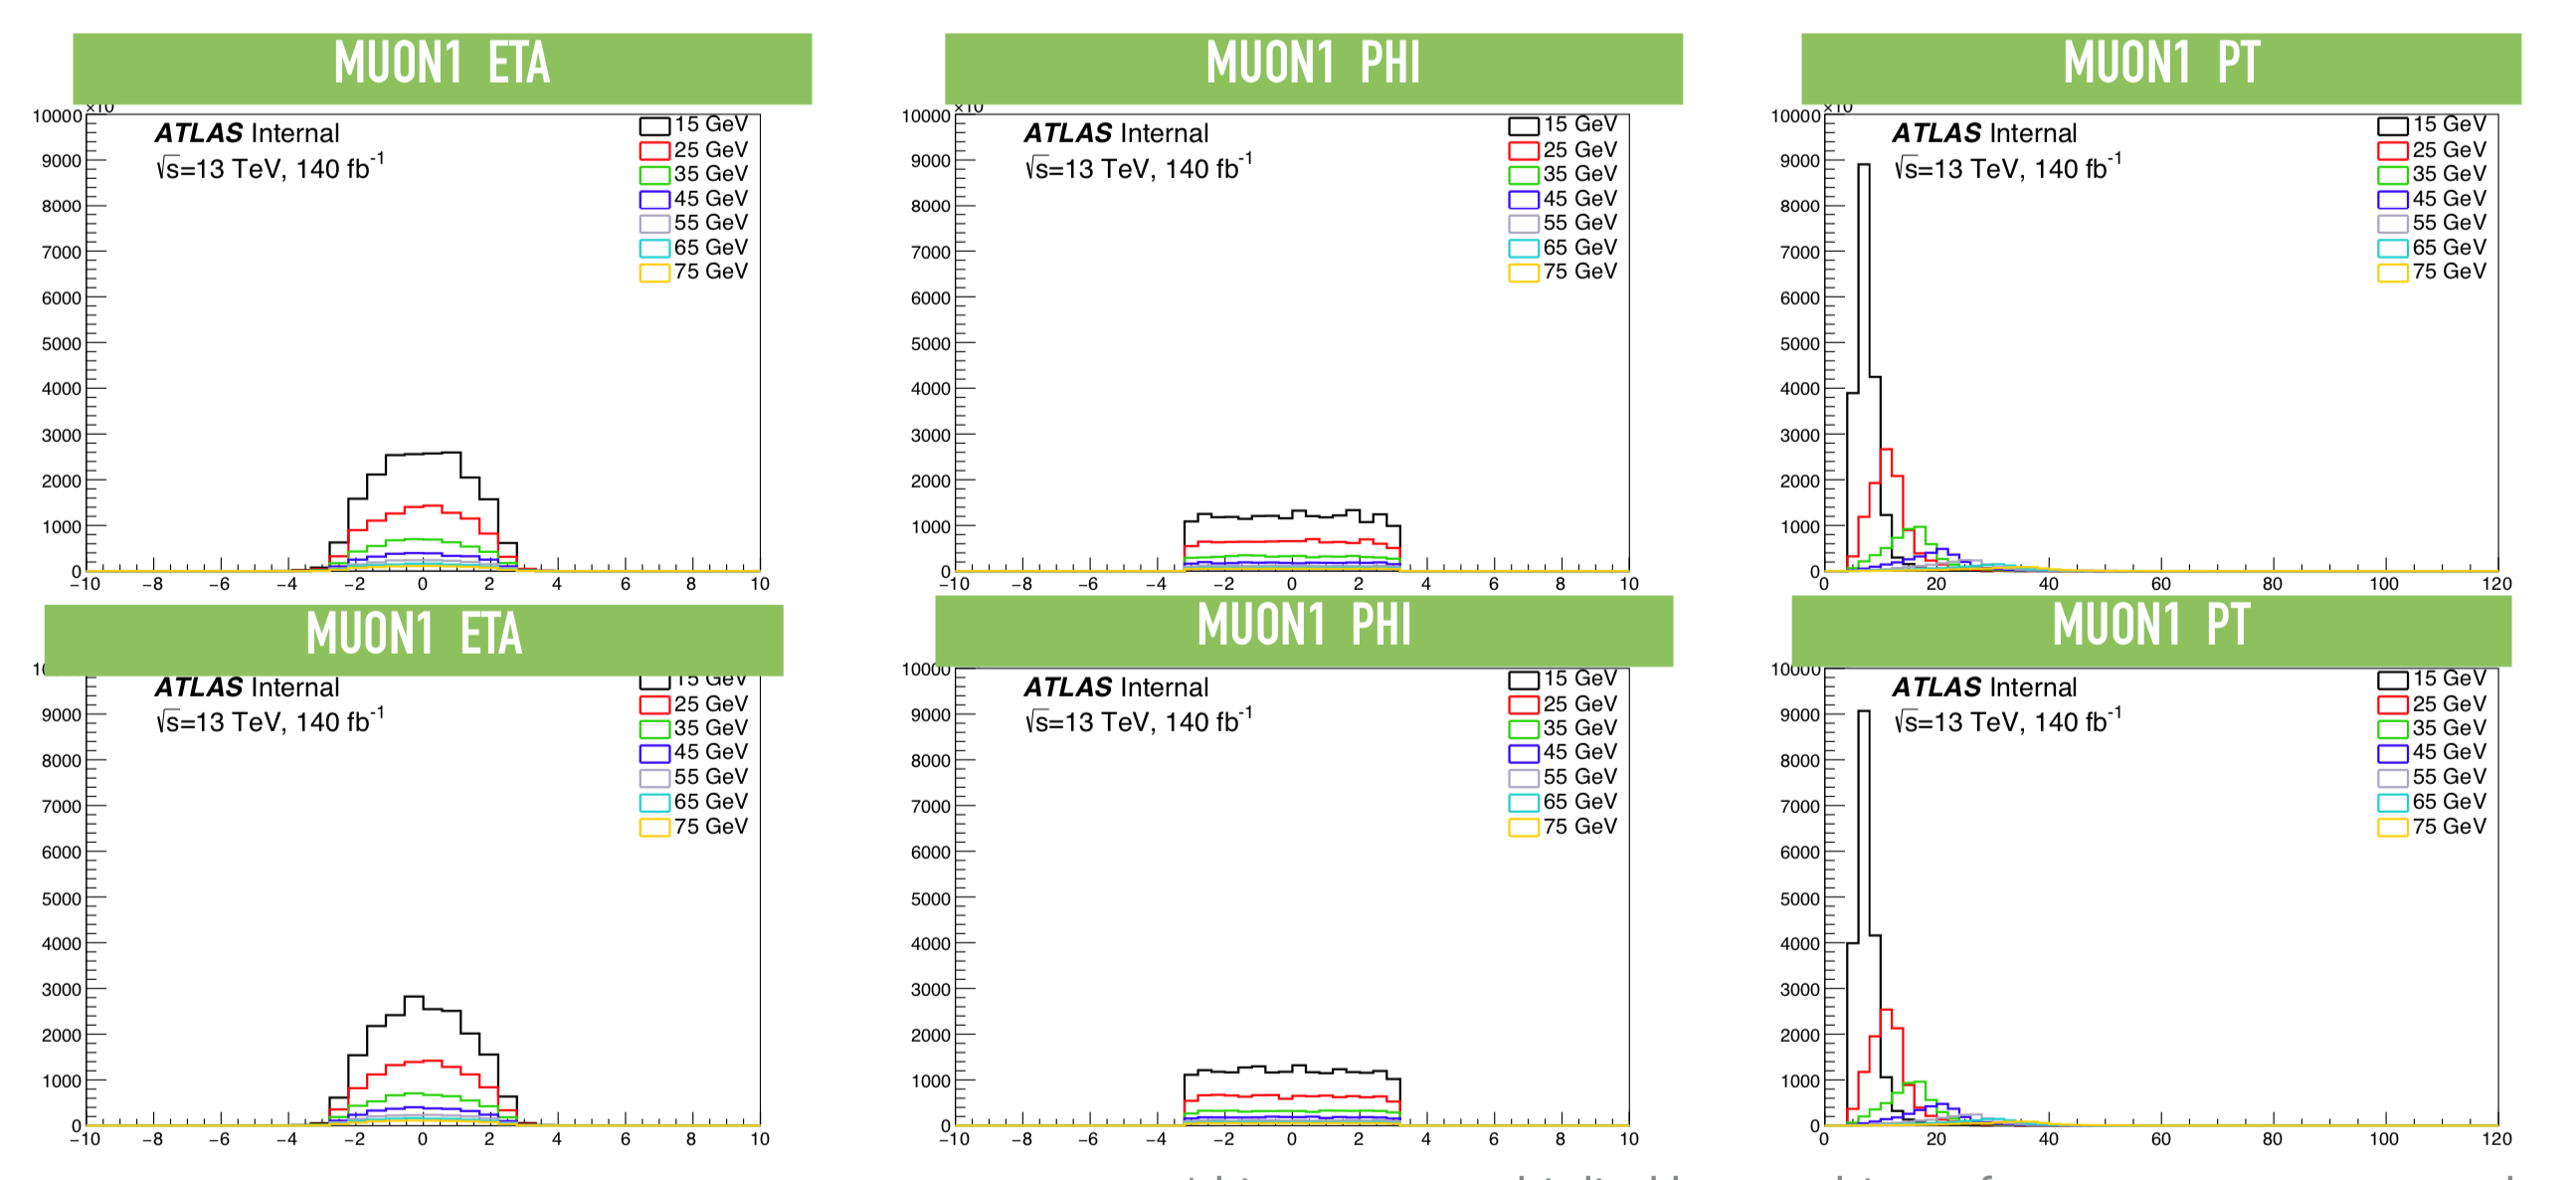
\includegraphics[width=0.75\textwidth]{figures/chapter_dimuon/dimuondist1}
%        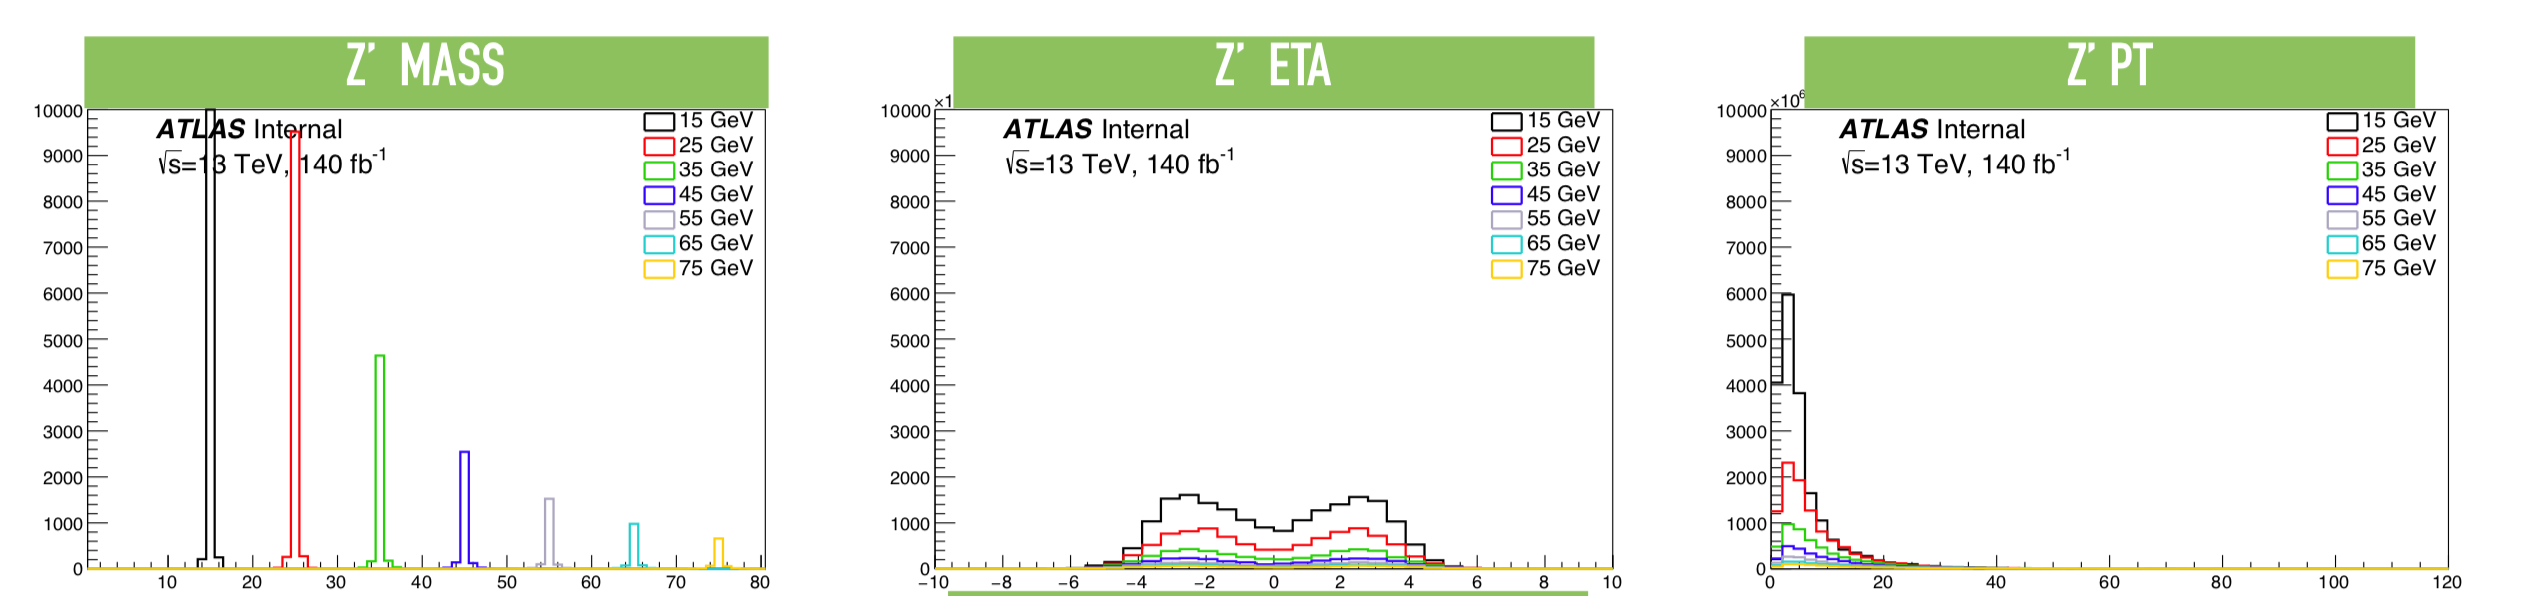
\includegraphics[width=0.75\textwidth]{figures/chapter_dimuon/dimuondist2}
%        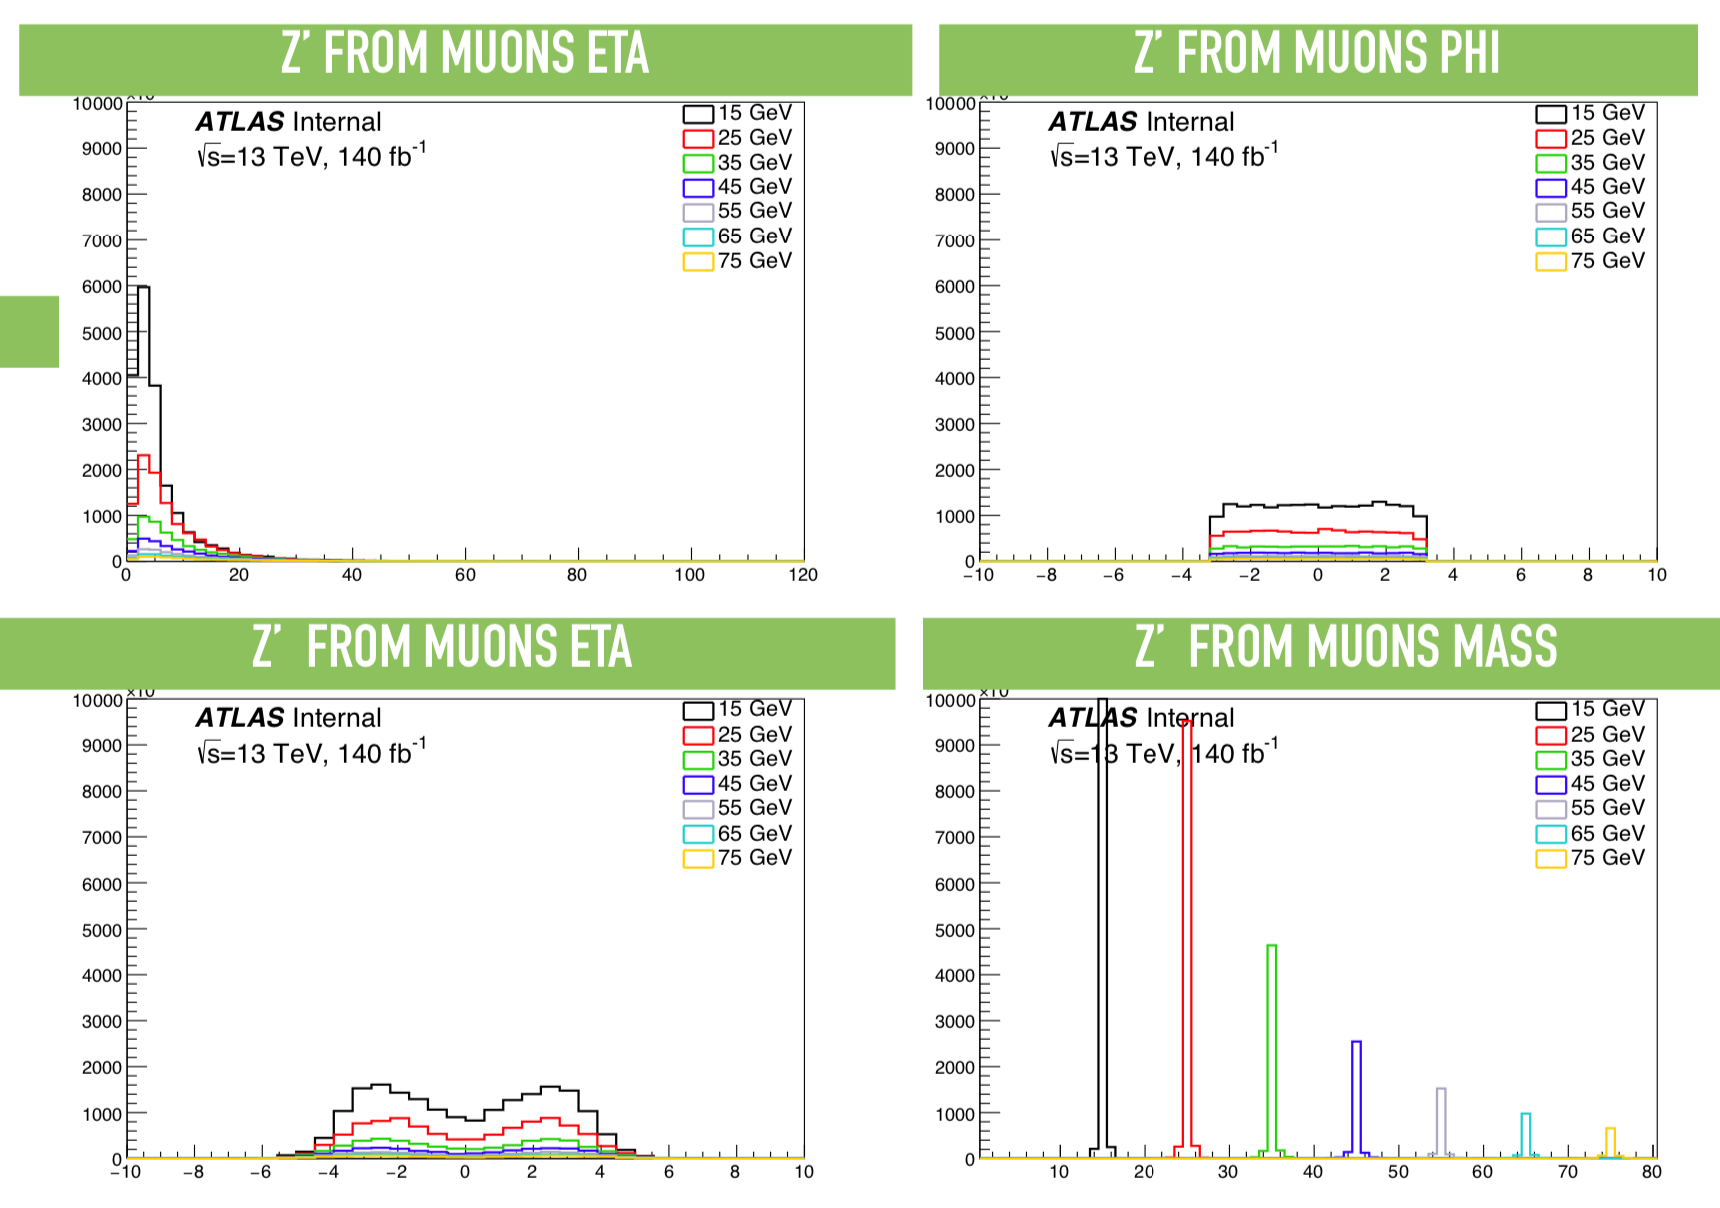
\includegraphics[width=0.5\textwidth]{figures/chapter_dimuon/dimuondist3}
%        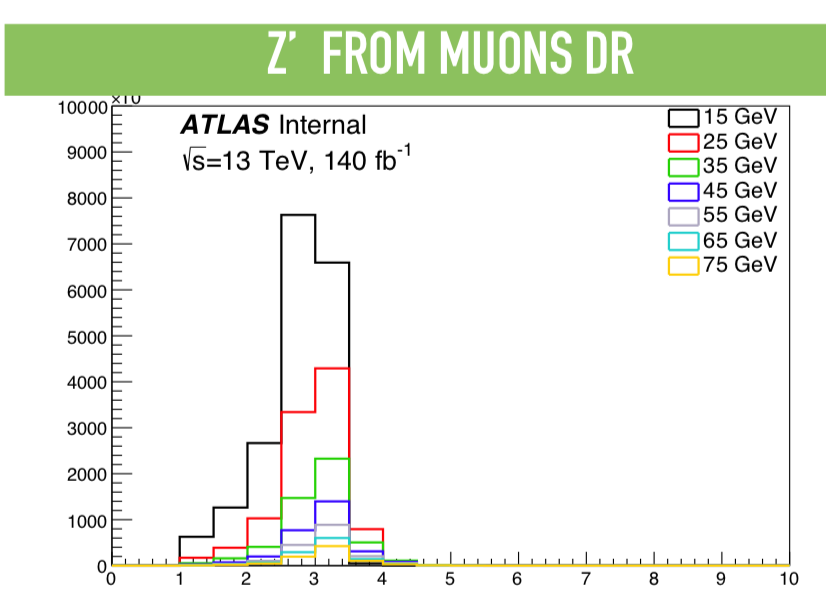
\includegraphics[width=0.2\textwidth]{figures/chapter_dimuon/dimuondist4}
%        \caption{
%        This figure shows the signal distribution of the inclusive dimuon samples generated. A minimal cut of muon pt >14 gev are done on the two leading muons. }
%        \label{fig:dimuon}
%    \end{center}
%\end{figure}


%\begin{figure}[!htb]
%    \begin{center}
%        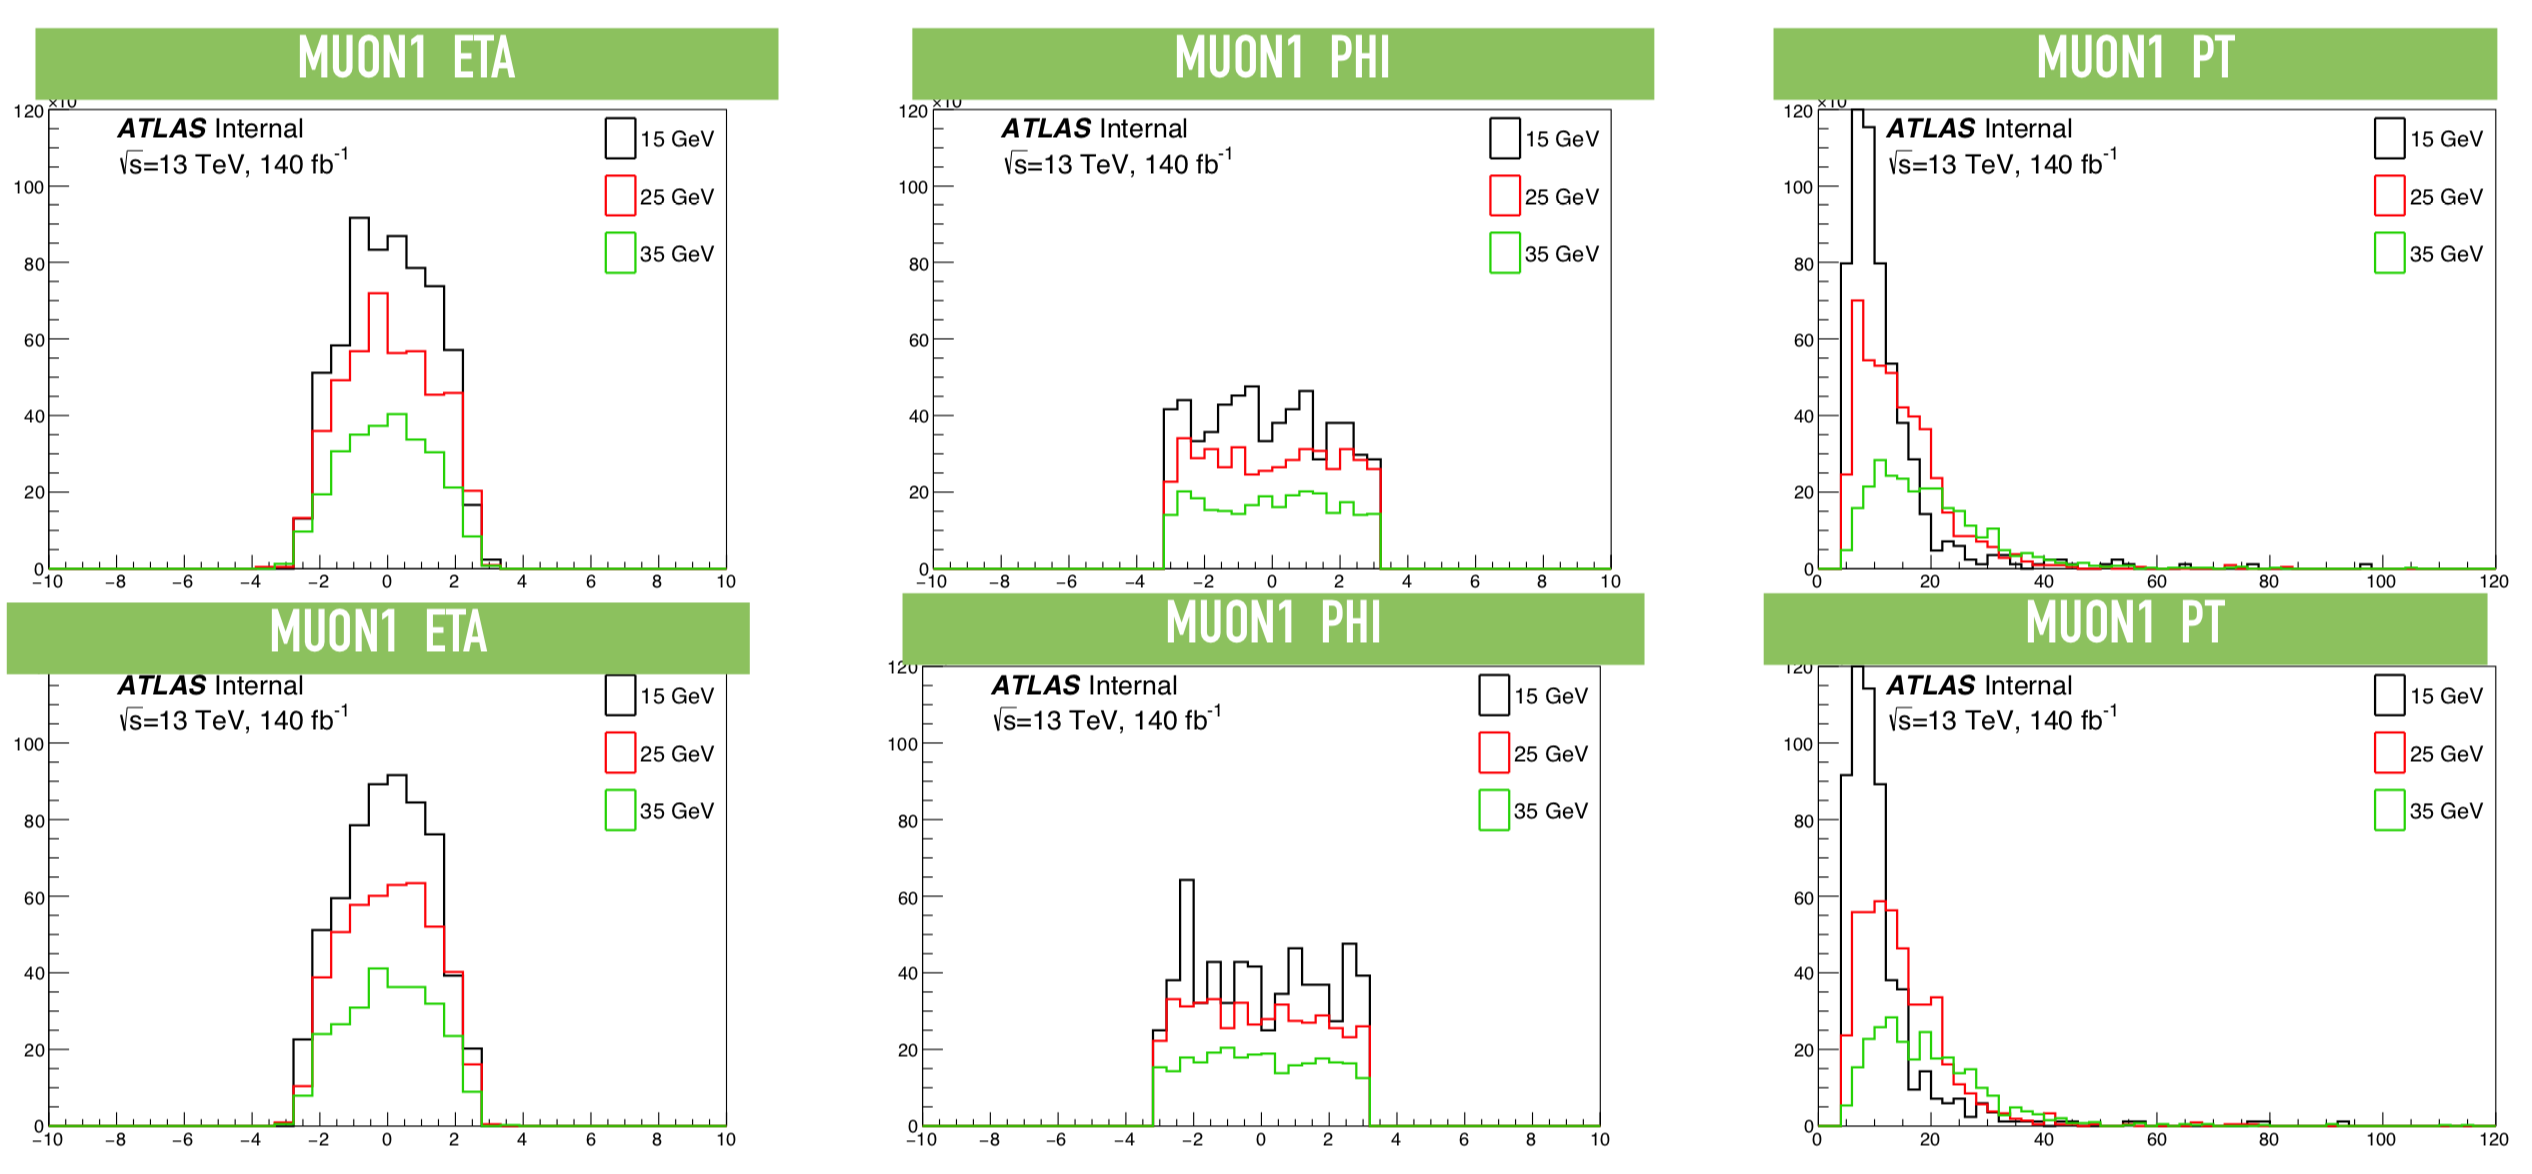
\includegraphics[width=0.75\textwidth]{figures/chapter_dimuon/dimuonISRdist1}
%        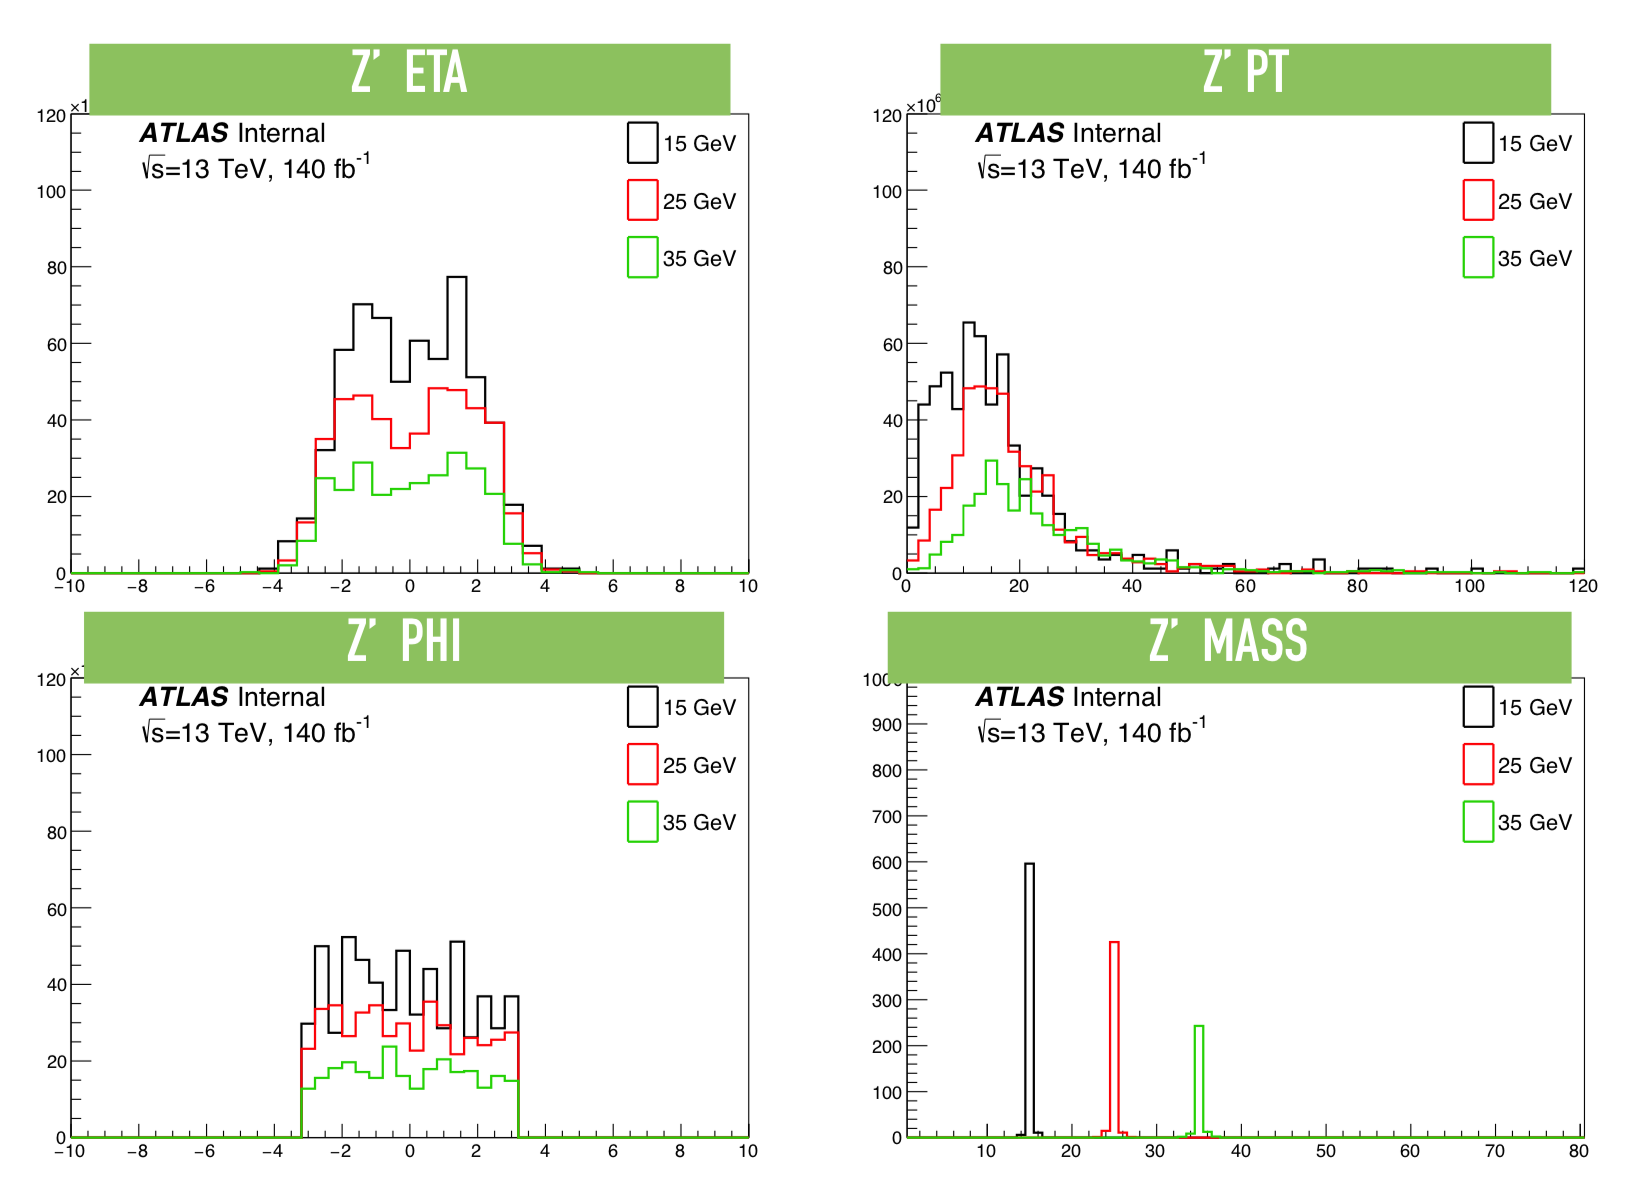
\includegraphics[width=0.5\textwidth]{figures/chapter_dimuon/dimuonISRdist2}
%        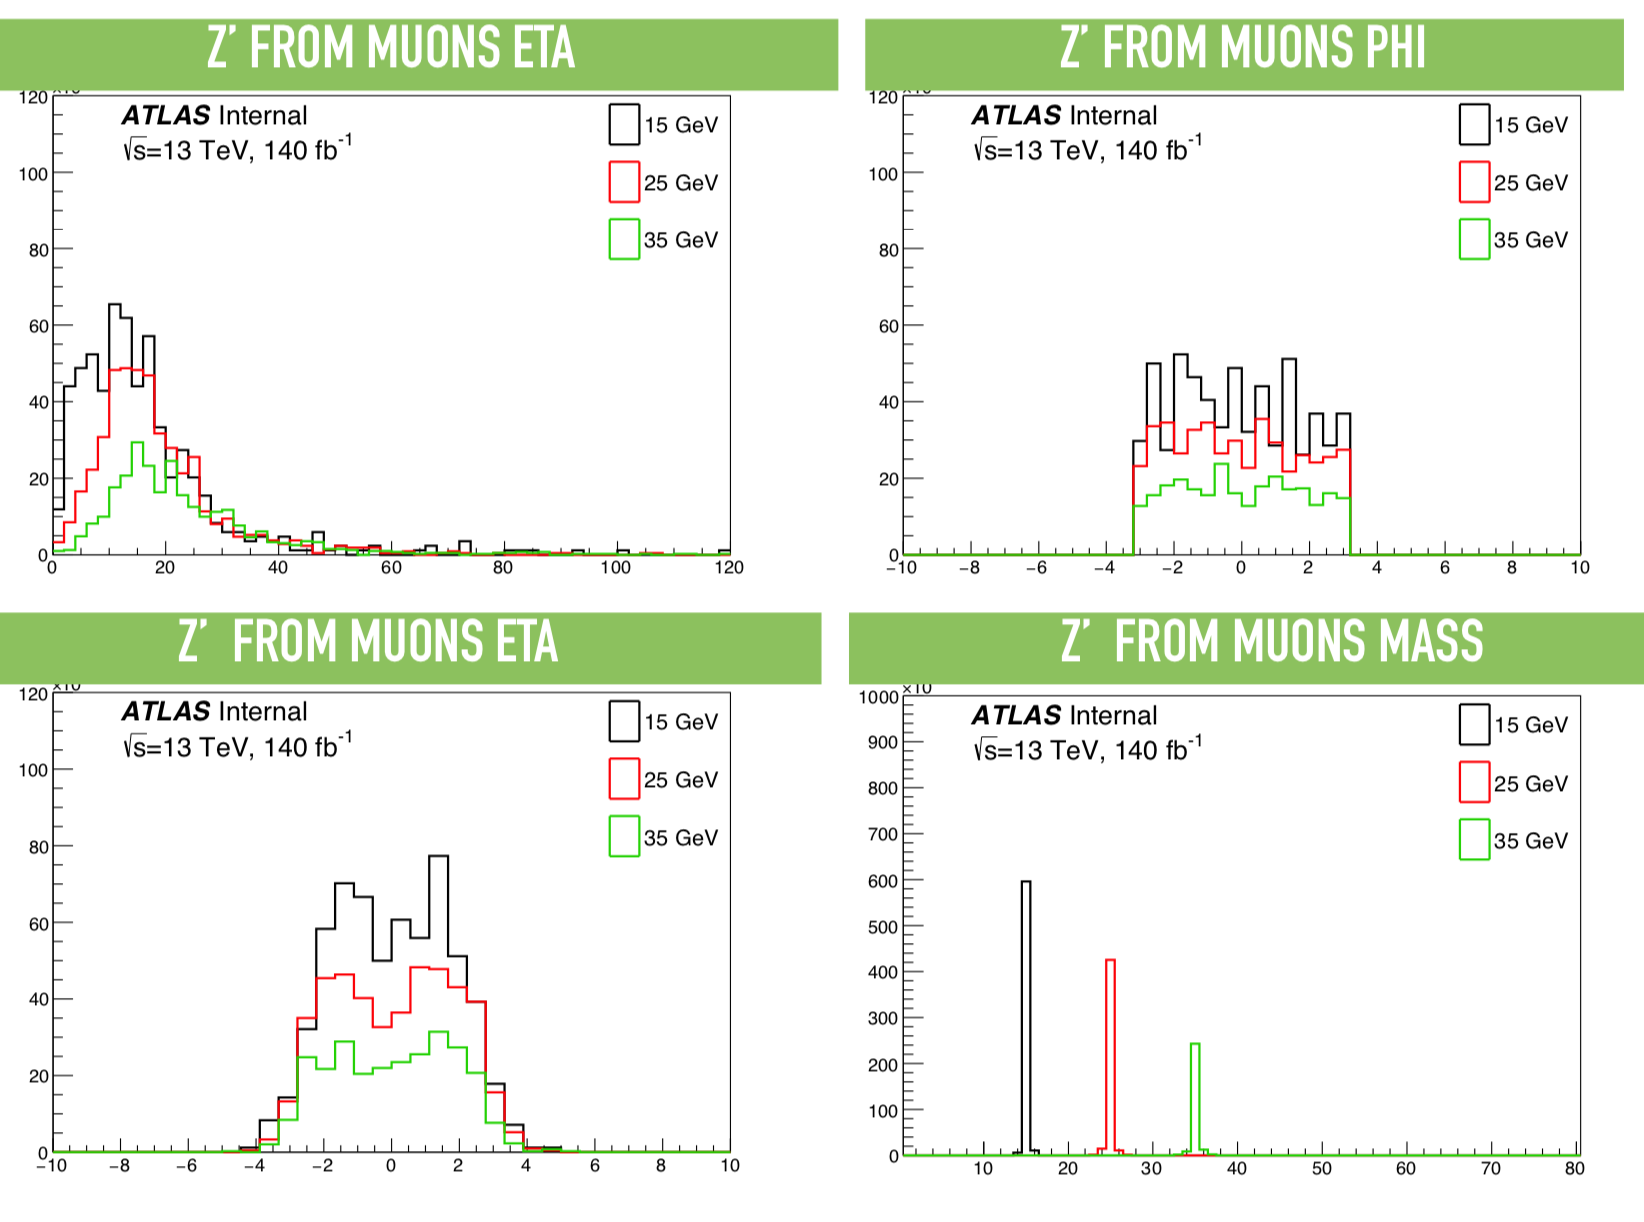
\includegraphics[width=0.5\textwidth]{figures/chapter_dimuon/dimuonISRdist3}
%        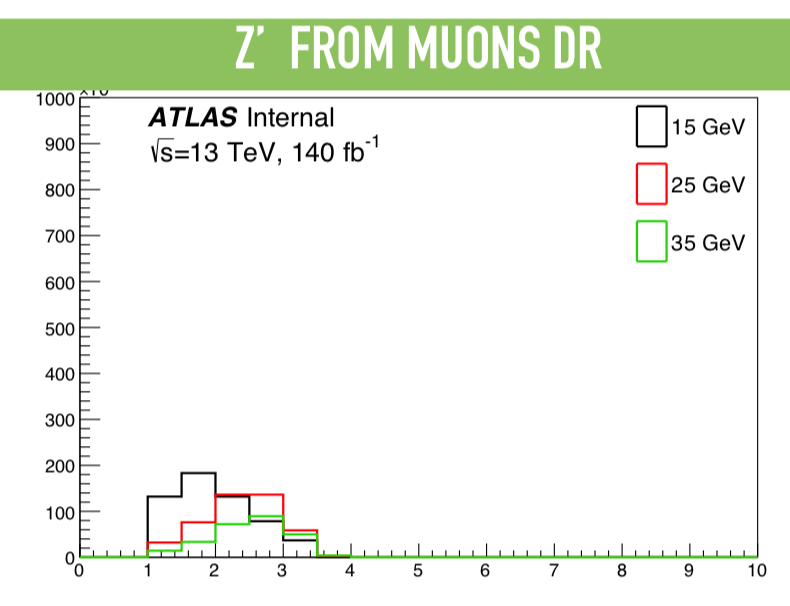
\includegraphics[width=0.2\textwidth]{figures/chapter_dimuon/dimuonISRdist4}
%        \caption{
%        This figure shows the signal distribution of the boosted dimuon samples generated. A minimal cut of muon pt >14 gev are done on the two leading muons. }
%       \label{fig:boosted}
%    \end{center}
%\end{figure}


\subsection{Trigger Chain}
\label{section:trigger}
Triggering is the selective storage and event for maximal processing efficiency. Details on the ATLAS triggering system can be found in Chapter~\ref{chapter:ATLAS}.
Triggering streams each have different cuts and they are tailored for different purposes, using multiple trigger stream with careful re-weighting could maximize the total event number for analysis. In the dimuon analysis, three trigger streams are employed for this reason.

\begin{table}[!htb]
    \begin{center}
    \caption{
        The table shows the trigger used for the dataset.
    }
\label{tab:Data Trigger}
\begin{tabular}{|l|l|l|l|l}
\hline
\textbf{Type}   & \textbf{Period}                                                         &\textbf{Trigger Chain} &\textbf{Level 1} &\textbf{$p_{T}^{\textrm{cut offline}}$}\\ \hline
Isolation Single Muon   & 2015 & HLT\_mu26\_iloose\_L1mu15 & MU15 & 27 \\ 
                        & 2016-2018  & HLT\_mu26\_ivarmedium    & MU20 & \\ \hline
Non-Isolated Single Muon & 2015-2018                                       &$HLT_mu50$& MU20& 27 \\ \hline
Symmetric Dimuon & 2015 & HLT\_2mu10 & 2MU10 & 15, 15 \\
                 & 2015-2018 & HLT\_2mu14 & 2MU10 & \\ \hline
Assymetric Dimuon & 2015 & HLT\_mu18\_mu8noL1 & MU15 & 24, 10 \\
                  & 2016-2018 & HLT\_mu22\_mu8noL1 & MU20 \\ \hline
\end{tabular}
\end{center}
\end{table}

\begin{figure}[!htb]
    \begin{center}
        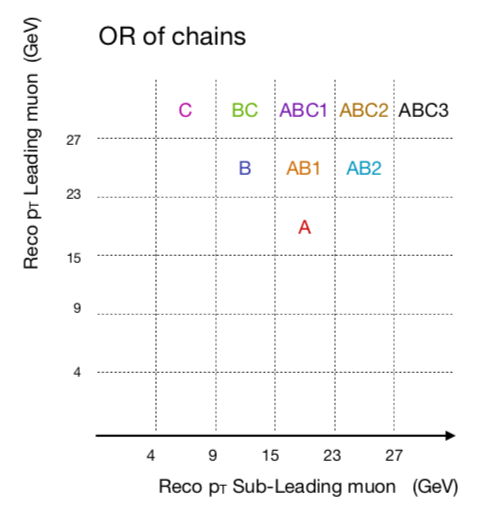
\includegraphics[width=0.45\textwidth]{figures/chapter_dimuon/TriggerChain}        
        \caption{
        This cartoon illstrate the trigger used for the different trigger region: A is HLT\_2mu14; B represents HLT\_mu22\_mu8noL1; C shows HLT\_mu26\_ivarmedium. }
    \end{center}
\end{figure}
\FloatBarrier

\section{Data preparation}
The final result of the strategies presented in this chapter are collected from proton-proton collision data during the ATLAS Run 2 period at a center-of-mass energy of $\sqrt{13}$ TeV from 2016-2018. The preliminary strategy of this chapter is generated from ATLAS full simulation Monte Carlo, besides the $Z > \mu \mu $ sample used. Due the process\'s low statistics in the ATLAS full simulation, a full size $Z > \mu \mu$ sample is created through a fast Sherpa and PYTHIA8 combination
generation at the truth level, where $P_{T}$ smearing is applied for detector effect. Section~\ref{sec:fastsimulation} details the superfast event generation.

\subsection{Samples Used for the Analysis}
The following are the samples used for the analysis. The largest background contribution in this analysis came from $Z > \mu\mu $ decay; the second largest contribution originates from $Z > \tau \tau$, other process including the t-channel $t\bar{t}$ , diboson decay as well as top decay also contribute a considerable amount to the background events.

\subsubsection{Fast Simulation $Z > \mu\mu$  Samples}
\label{sec:fastsimulation}
Due to the low statistics in the primary background sample in  $Z \> \mu \mu$, fast generation relying on Pythia8 and a smearing function for the detector effect has been used to emulate the statistical fluctuation of the full dataset. Four different variation of the superfast statistics as been used, each uses a different pdf set for the generator tuning. The Nominal set uses the ATLAS A14 NNPDF2.3LO; the down variation and up variation uses the variation tune parameters Var3C listed
here~\cite{ATL-PHYS-PUB-2014-021}; whereas the $\eta$ variation uses ATLAS A15 NNPDF2.3 along with QCD and QED NLO. More details on the fast simulation can be found here~\ref{Artoni:2703492}.

\begin{table}[!htb]
    \begin{center}
    \caption{
        The table shows the Monte Carlo background dataset used for the analysis. 
    \label{table:MC}
    }
\label{tab:MC samples}
\begin{tabular}{|l|l|l|}
\hline
\textbf{MC Type}   & \textbf{DSID}                                                         &\textbf{Generator Used}\\ \hline
Z+ jets $\mu\mu$   & 364100 - 364113 , 364198-364203                                       &Fast Simulation through PYTHIA\\ \hline
Z+jets $\tau \tau$ & 364128 - 364141 , 364210-364215                                       &Sherpa\\ \hline
$t\bar{t}$         & 410472                                                                &Sherpa\\ \hline
Diboson            & 364253 - 364255 , 363355 - 363360 ; &Sherpa \\
& 363489 ; 364250 ; 364288 - 364290 & \\ \hline
Top decay          & 410644 - 410645 , 410658 - 410659 ;                   &Powheg+Pythia8\\ 
&410648 - 410649 & \\ \hline
$W + jets \mu\nu$  & 364156 - 364169                                                       &Sherpa\\ \hline
$b\bar{b}$         & 363833                                                                &Pythia8b\\ \hline
$c\bar{c}$         & 363834                                                                &Pythia8b\\ \hline
\end{tabular}
\end{center}
\end{table}

In addition to sources in this table, QCD fakes that may contribute to background events are estimated by same-signed dimuon pairs in data that satistfy all other event requirements. The rational is that in data all of the same-signed dimuon would all come from QCD contribution, and that the contribution amount would be equal to the opposite-signed contribution of fakes from QCD. Figure~\ref{fig:samesigned} shows a background composition plot with the same signed contribution subtracted out. The fake QCD contribution makes up less than 1\% of all the events. After the application of the Fake estimation, the overall agreement between data and MC in controlled regions are within acceptable range, it shows that the MC is ready to be used for statistics strategy studies.

\begin{figure}[!htb]
    \begin{center}
        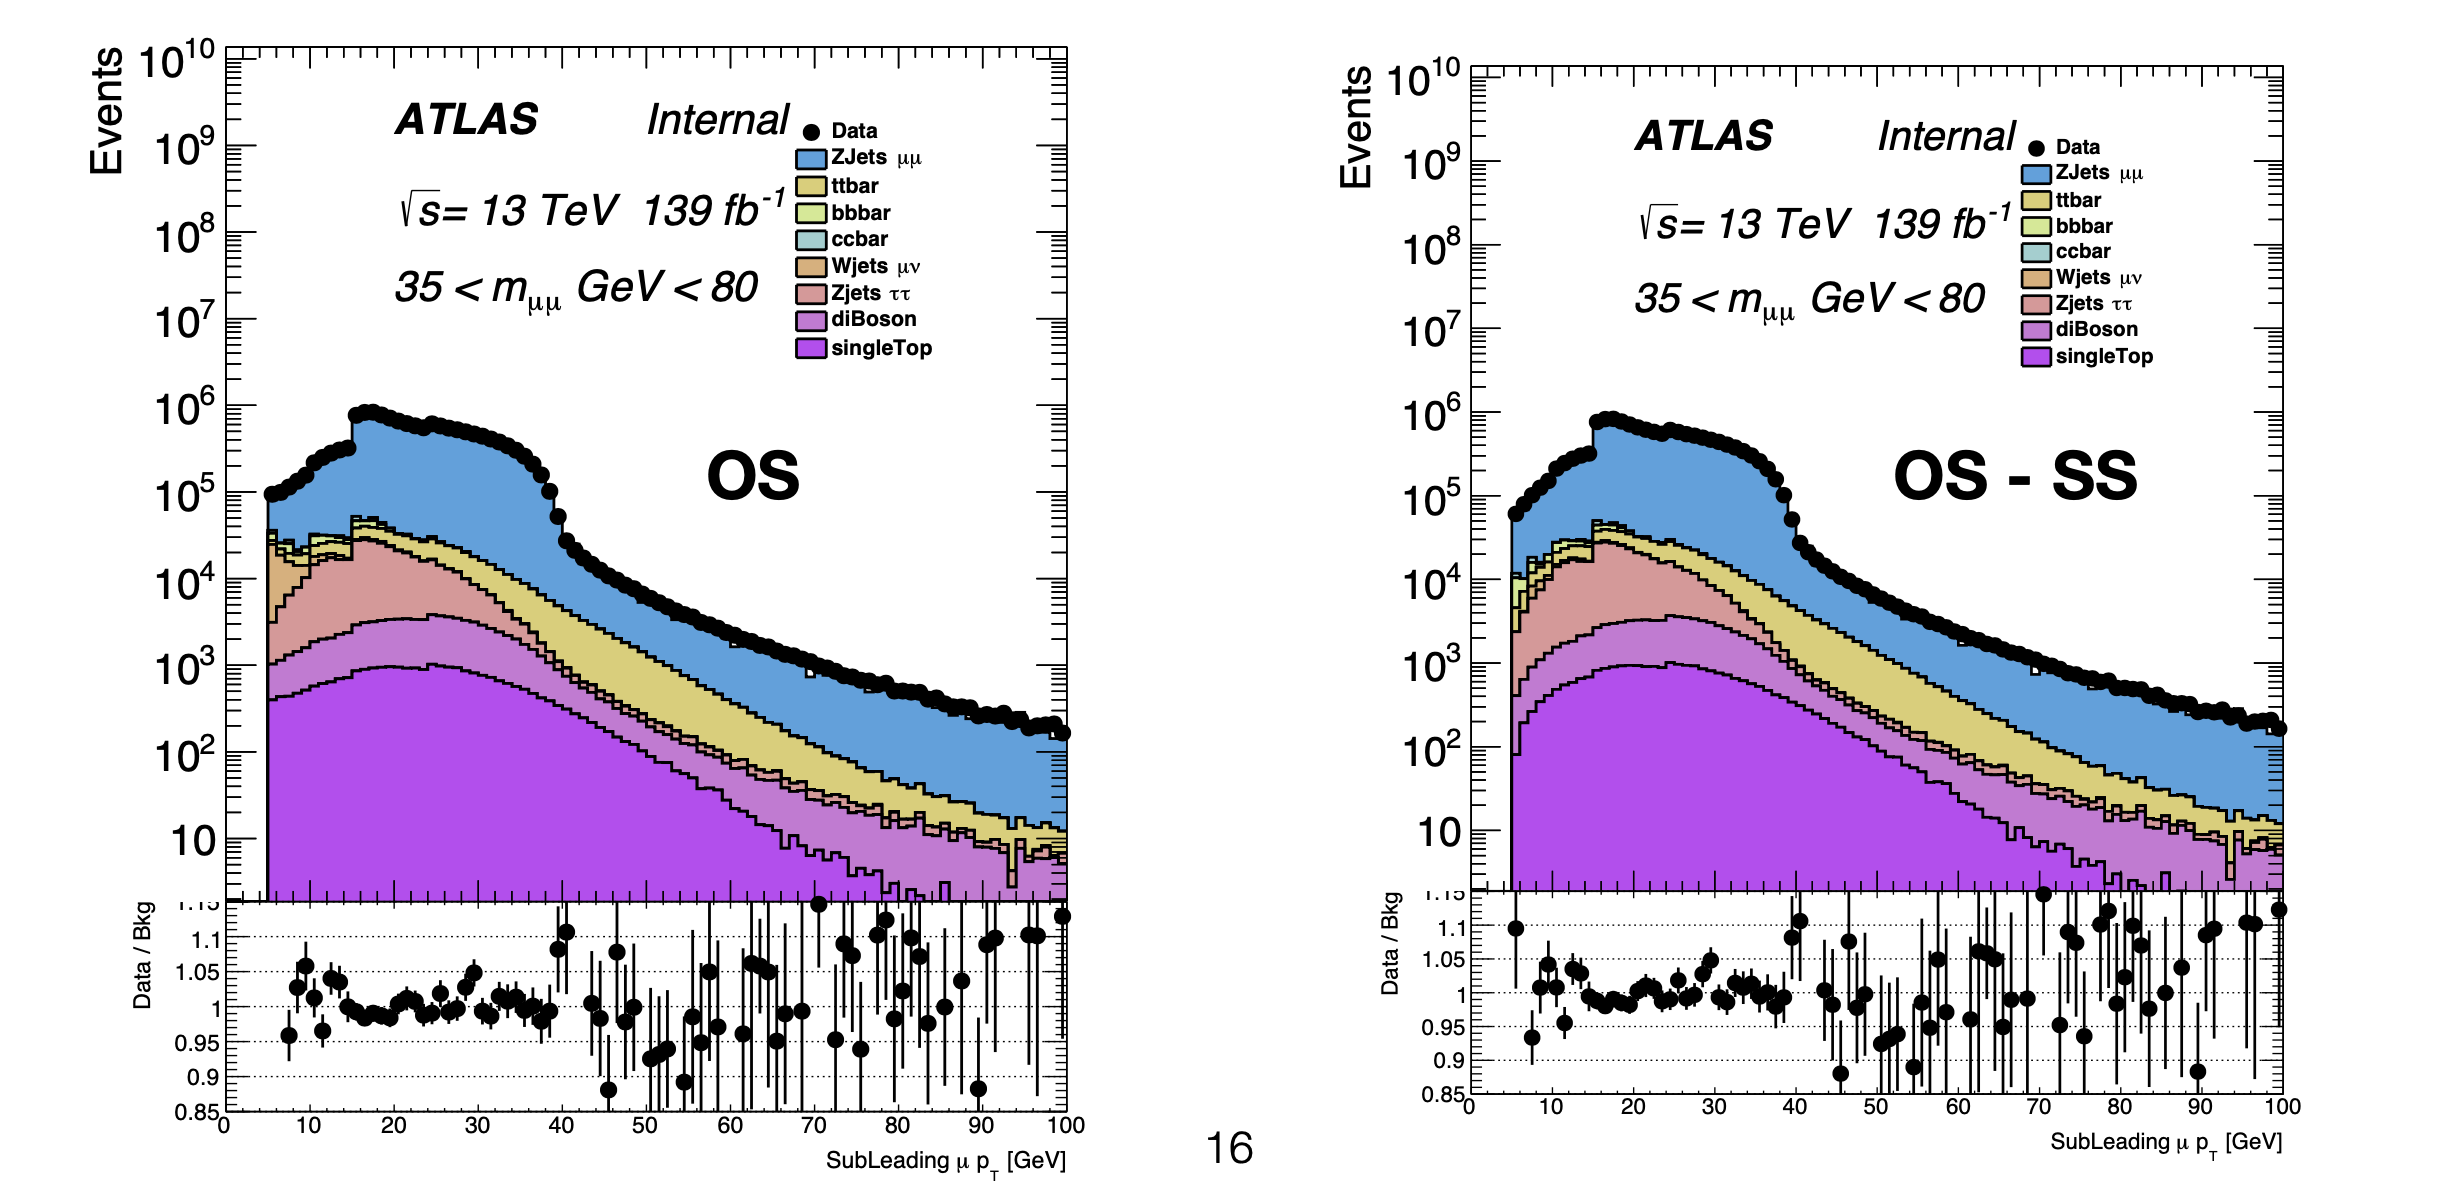
\includegraphics[width=0.85\textwidth]{figures/chapter_dimuon/samesigned}
        \caption{
        These plots shows the leading muon transverse momentum distribution and the subleading muon transverse momentum distribution with the super fast simulation.  }
        \label{fig:samesigned}
    \end{center}
\end{figure}
\FloatBarrier

In the analysis, studies was done and it was found that muons of the \textbf{MEDIUM} working point and the \textbf{FixedCutPFlowLoose} isolation working point (Defined in Chapter~\ref{chapter:common_analysis_items}) will provide the maximum signal sensitivity and muon performance. Two muons of at least 4 GeV in tranverse momentum are required for each event. In addition, $|\eta|< 2.5$ is required for both muons. An additional $P_{T}> 14GeV$ cut is applied to events in the boosted channel.

\begin{figure}[!htb]
    \begin{center}
        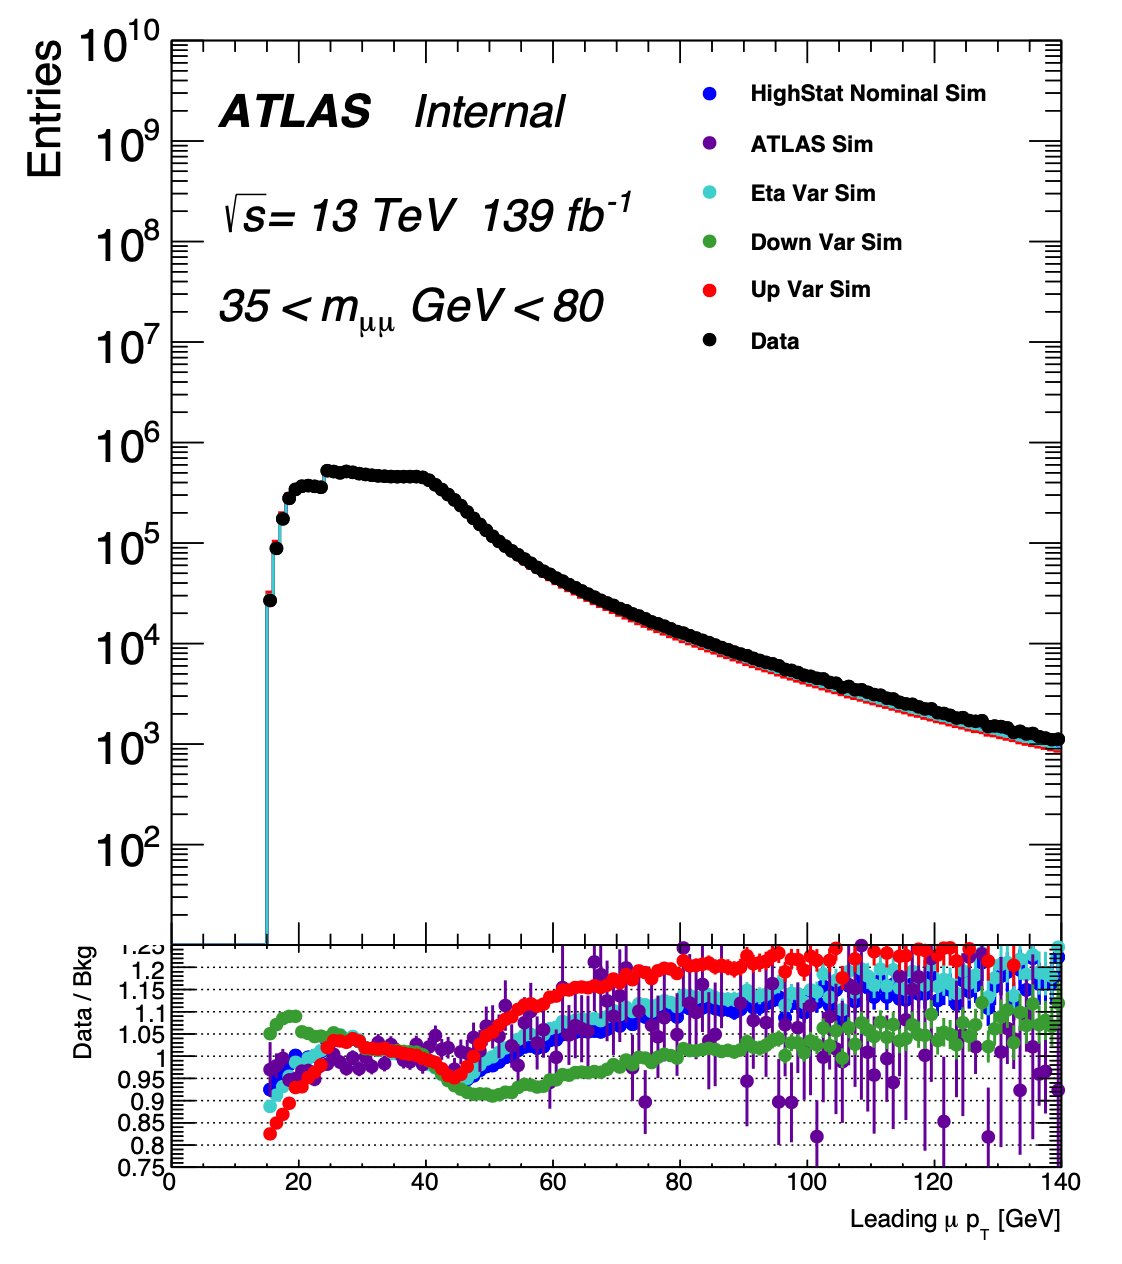
\includegraphics[width=0.45\textwidth]{figures/chapter_dimuon/superfast_leadingMuonPT}
        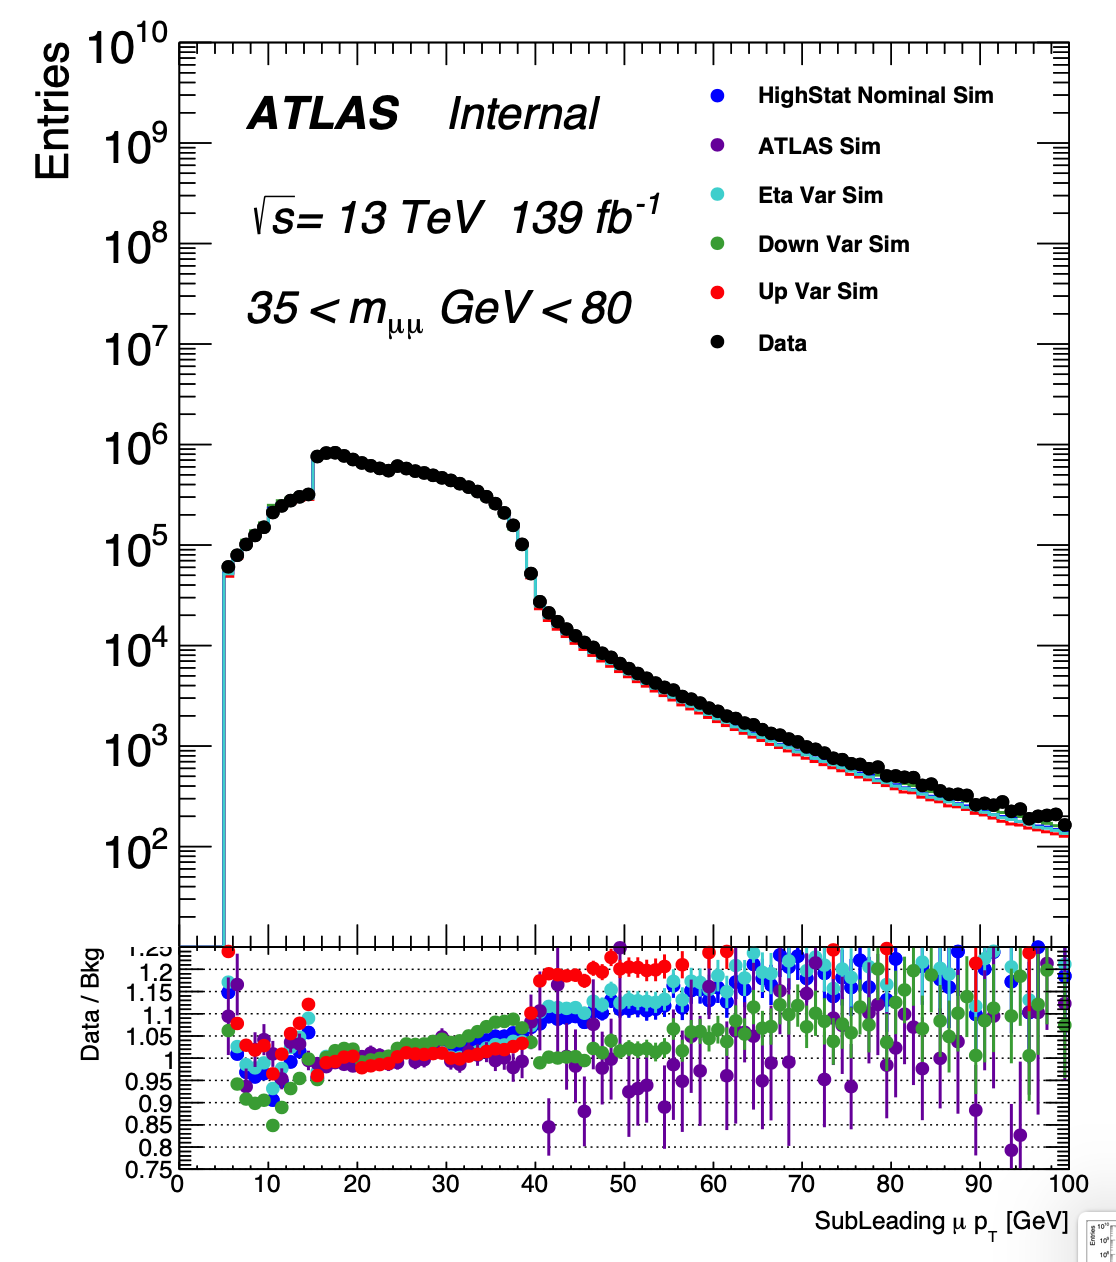
\includegraphics[width=0.45\textwidth]{figures/chapter_dimuon/superfast_subleadingMuonPT}
        \caption{
        These plots shows the leading muon transverse momentum distribution and the subleading muon transverse momentum distribution with the super fast simulation.  }
    \end{center}
\end{figure}
\FloatBarrier


%\begin{table}[!htb]
%    \begin{center}
%    \caption{
%        The table shows the Data dataset used for the analysis. 
%    }
%\label{tab:MC samples}
%\begin{tabular}{|l|l|}
%\hline
%\textbf{Data Taking year}   & \textbf{Data Period} \\ \hline
%2015   & D-J                                       \\ \hline
%2016   & A-L                                       \\ \hline
%2017   & B-F, H                                    \\ \hline
%2018   & B-F, I, K, L-O, Q                         \\ \hline
%\end{tabular}
%\end{center}
%\end{table}



%The efficiency are calculated for each region for the subsequent weighting of in the trigger scale factor.
%\begin{equation}
%    SF= \epsilon_{data}/\episilon_{MC}
%\end{equation}

%\subsection{Background composition}
%The background composition of the Monte Carlo is shown here:
%
%\begin{figure}[!htb]
%    \begin{center}
%        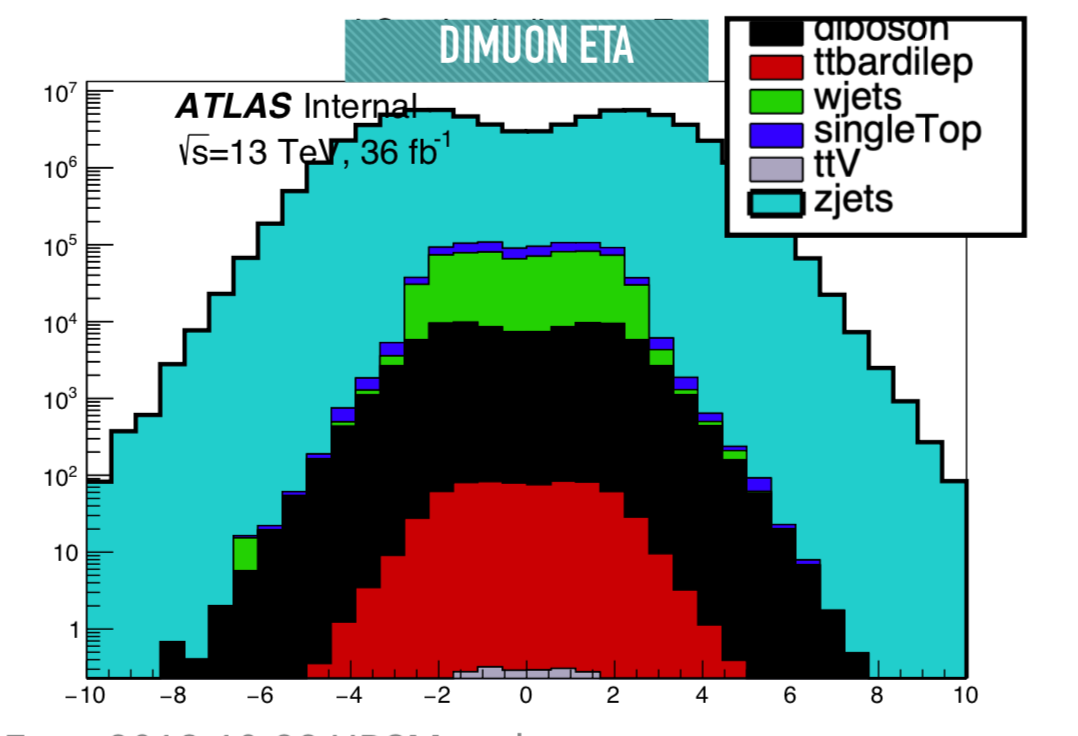
\includegraphics[width=0.75\textwidth]{figures/chapter_dimuon/backgroundcomposition}
%        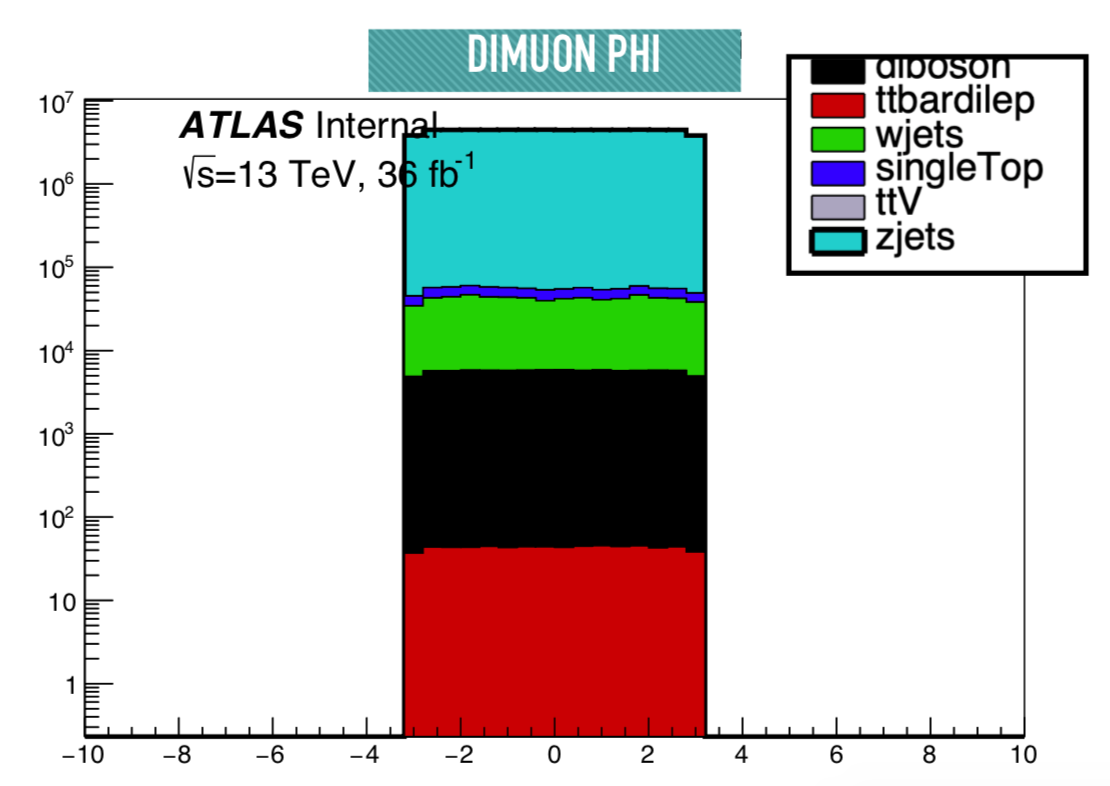
\includegraphics[width=0.75\textwidth]{figures/chapter_dimuon/backgroundcomposition2}
%        \caption{
%        This cartoon illstrate the background composition of the samples }
%    \end{center}
%\end{figure}

%\subsection{Event Selection}
%Following the above trigger cuts, the following event selections are made on the muons:
%
%\subsubsection*{Muon Working Point}
%The medium working point is chosen for the muons, details to the working point can be found here: 
%
%The choice is made on the medium working point over low PT, as the trigger threshold effectively cut out most muons below 8GeV. The Low PT working point only has a higher efficiency over the medium working point below  6 GeV. 

%\subsubsection*{Isolation Working Point}
%FixedCutPflowLoose is chosen to be the isolation working point, details on the working point description can be found here:~\ref{}. 

%\subsubsection{Fake Estimation}
%Fakes are objects that are not opposite signed dimuon pairs that falls into the selection requirement in data event selection due to misidentifications.
%Since the fakes mainly comes from QCD ATLAS processes, the amount from same signed process and opposite signed process are approximately the same. 
%Fakes in the background sample can be estimated from the same signed leptons in data. Studies found that the content is less than 1\% of all the background contribution. The estimated same signed leptons contribution is added to the MC background composition.
%
%\begin{figure}[!htb]
%    \begin{center}
%        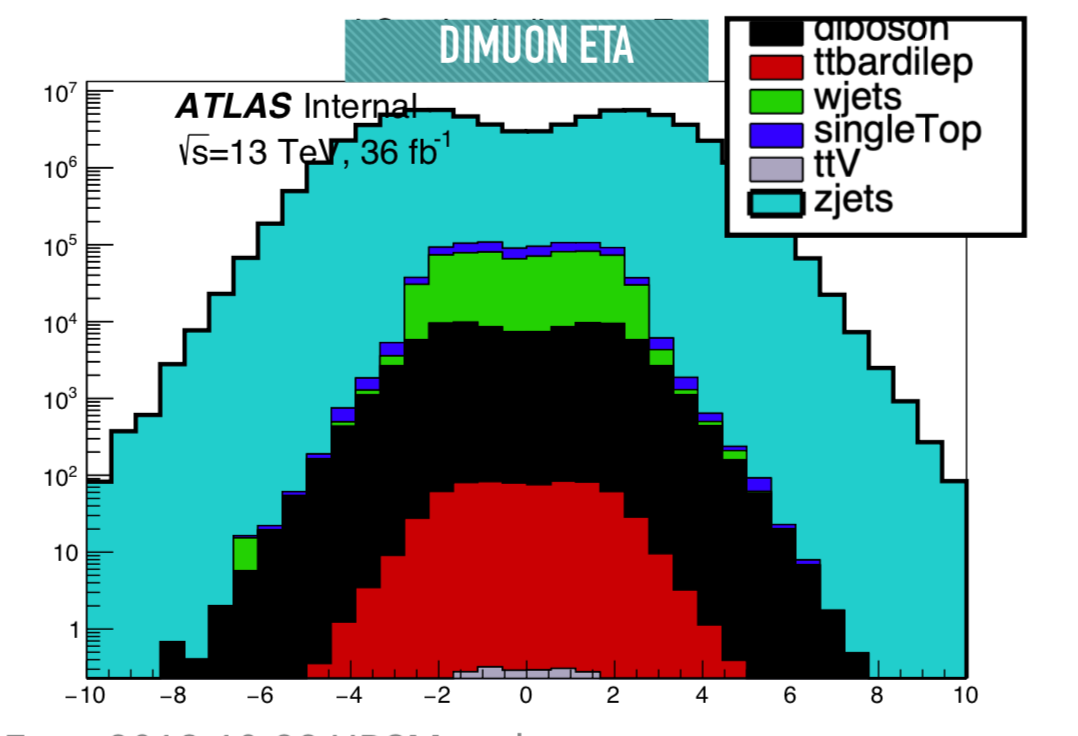
\includegraphics[width=0.75\textwidth]{figures/chapter_dimuon/backgroundcomposition}
%        \caption{
%        This cartoon illstrating the amount of fakes in the background composition. SS refers to same signed lepton in the data sample set, whereas OS refers to the opposite sign lepton pairs in data. }
%    \end{center}
%\end{figure}


\subsection{Dimuon Mass Spectrum Resolution}
To define the binning of the dimuon mass distribution in the signal region, the dimuon mass resolution is studied. The following study is done on the Z > $\mu \mu$. Detail on the procedure can be found in Chapter~\ref{chapter:common_analysis_items}.
A Gaussian distribution fit is performed on the resonance mass $m_{\mu\mu_{Truth}} - m_{\mu\mu{Reco}}$ quantity. From the fit, the width of the Gaussian is obtained~\ref{fig:fit}, and is taken to be the detector resolution in the dimuon mass distribution. The bin-by-bin resolution result is shown in Figure~\ref{fig:sigma}.
    

\begin{figure}[!htb]
    \begin{center}
        \includegraphics[width=0.45\textwidth]{figures/chapter_dimuon/fitError}        
        \caption{
            A Gaussian distribution fit is made on the the difference between the truth dimuon resonance mass and the reconstructed dimuon resonance mass.    }
    \end{center}
\end{figure}
\FloatBarrier
   
\begin{figure}[!htb]
    \begin{center}
        \includegraphics[width=0.45\textwidth]{figures/chapter_dimuon/sigma}        
        \caption{
        From the fitted Gaussian distribution, the width is obtained for different resonance mass. They are plotted here. The width-to-mass resolution $\sigma_{m_{\mu\mu}}/m_{\mu\mu}$ is found to be close to 1.5\%.}
    \end{center}
\end{figure}
\FloatBarrier


\subsection{Binning Strategy}
Using the resolution of the study from the last section and the mass distribution given in the theoretical signal section, the overall binning is chosen to be 0.25 GeV. Uniform binning simplified the fitting procedure considerably. The choice is also made out of consideration to ensure all signal searched for are at least 2 bin wide to reduce the probability of capturing a signal from statistical fluctuation only seen in one bin.

%\subsubsection{MC/Data Comparison}
%A detailed description on the MC/Data comparison test can be found here,\ref{sec:MCData}.  
%The agreement is shown to be good between the prepared MC and data. It shows that the MC is ready to be used for the subsequent tests.
%
%\begin{figure}[!htb]
%    \begin{center}
%        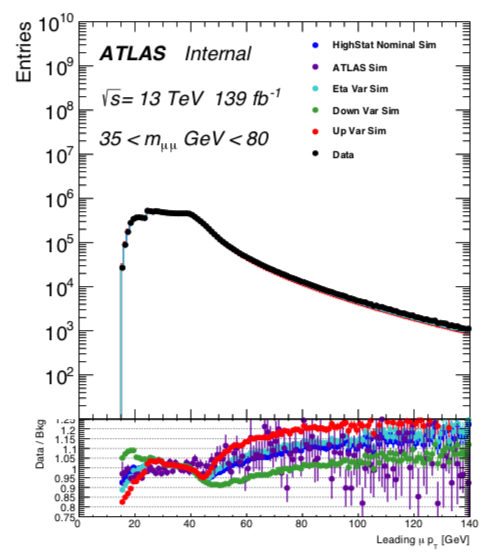
\includegraphics[width=0.75\textwidth]{figures/chapter_dimuon/MCDataCompare}
%        %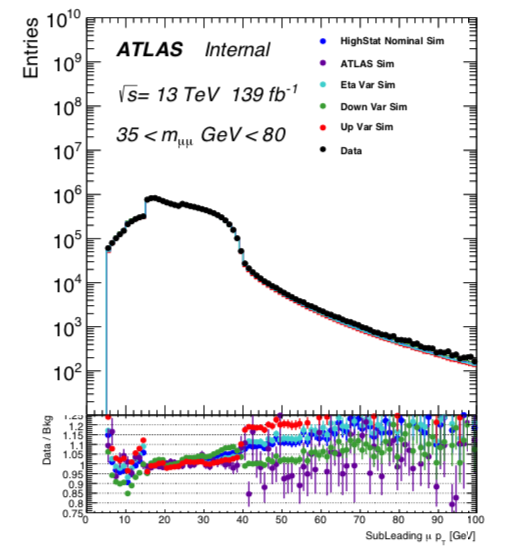
\includegraphics[width=0.75\textwidth]{figures/chapter_dimuon/MCDataCompare2}
%        %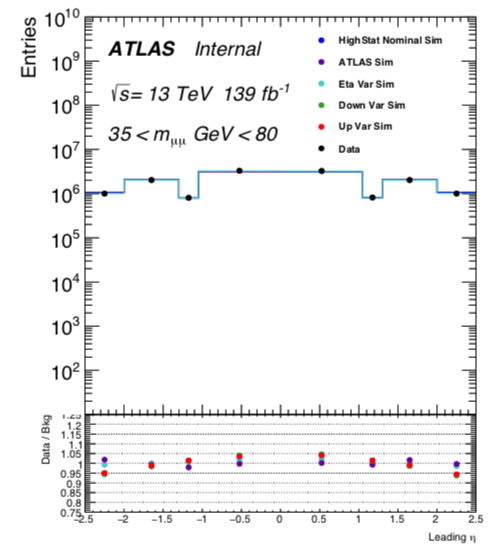
\includegraphics[width=0.75\textwidth]{figures/chapter_dimuon/MCDataCompare3}
%        %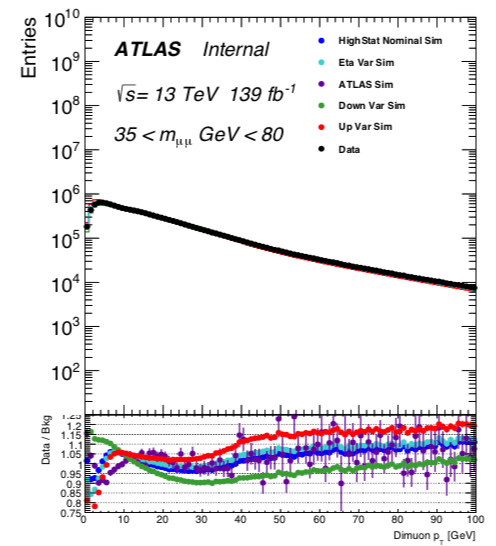
\includegraphics[width=0.75\textwidth]{figures/chapter_dimuon/MCDataCompare4}
%        %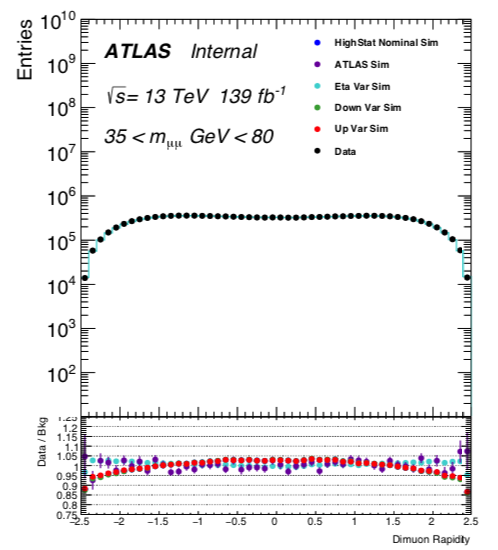
\includegraphics[width=0.75\textwidth]{figures/chapter_dimuon/MCDataCompare5}
%        \caption{
%        Monte Carlo and data comparison. A reasonable agreement is seen. Showing that the MC is ready to be used for the subsequent studies.
%        }
%    \end{center}
%\end{figure}

\section{Background Fitting}
As the fully simulated ATLAS MC for the background processes listed in table~\ref{table:MC} are neither reliable in shape or enough in count, the background fitting of the dimuon analysis relies on a data driven approach. Detail on data driven approaches for smooth background estimation is fully reviewd in Chapter~\ref{chapter:analysismethod}. The approach used by the dimuon analysis is the Gaussian Process approach outlined in Chapter~\ref{chapter:analysismethod}. Details specific to the analysis and results are detailed here.

\subsection{The Kernel}
The Gaussian process background and signal kernels used for this particular analysis method is given here~\ref{}. In Gaussian Process, the mean function prediction and the covariance function on the prediction variance are determined by the kernel function. (See details in Chapter~\ref{}.)

\begin{itemize}
    \item \textbf{Background Kernel} \textit{-``Radial Basis Function + White Noise Kernel"}
        \begin{equation}
                K_{bkg}(x, x') = A_{1} * exp(-\frac{||x-x'||}{2\sigma^{2}}) 
        \label{eq:backgroundkernel}
        \end{equation}

    Here, $A_{1}$ is the amplitude hyperparameter that describes the size of the kernel, $\sigma_{1}$ is the lengthscale parameter.
\item \textbf{Signal Kernel} \textit{- ``Exponential Center Kernel + White Noise Kernel "}
            \begin{equation}
            K(x_{i}, x_{j})=A_{2}\cdot exp(-(x-m)^{2}/(2\cdot\sigma_{2}^{2}))\cdot exp(-((x'-m)^{2}/(2\cdot\sigma_{2}^{2})))
            \label{eq:signalkernel}
            \end{equation}
\end{itemize}

    Here, $A_{2}$ is the amplitude of the signal kernel, m is the value where the kernel peaked on, and $\sigma_{2}$ is the lengthscale of the signal kernel. 

\subsubsection{Test for the Background Kernel}
Verification are done to ensure the background MC can be described by the background kernel. The procedure is described as the following: Toy distribution are created from drawing the Poissonian distribution in each bin. 10,000 new toy distributions are formed. Each are fitted with the Gaussian Process background kernel and test statistics defined in Section\ref{} are calculated for each fit. The test statistics of the original fit to the background MC is compared against the test statisitics of
the toy distribution to calculated the p-value. Results in Figure~\ref{fig:nominalstats} that all three test statistics tested the p-value is above 0.01 and that the kernel captures features in background distribution well. 

\begin{figure}[!htb]
    \begin{center}
        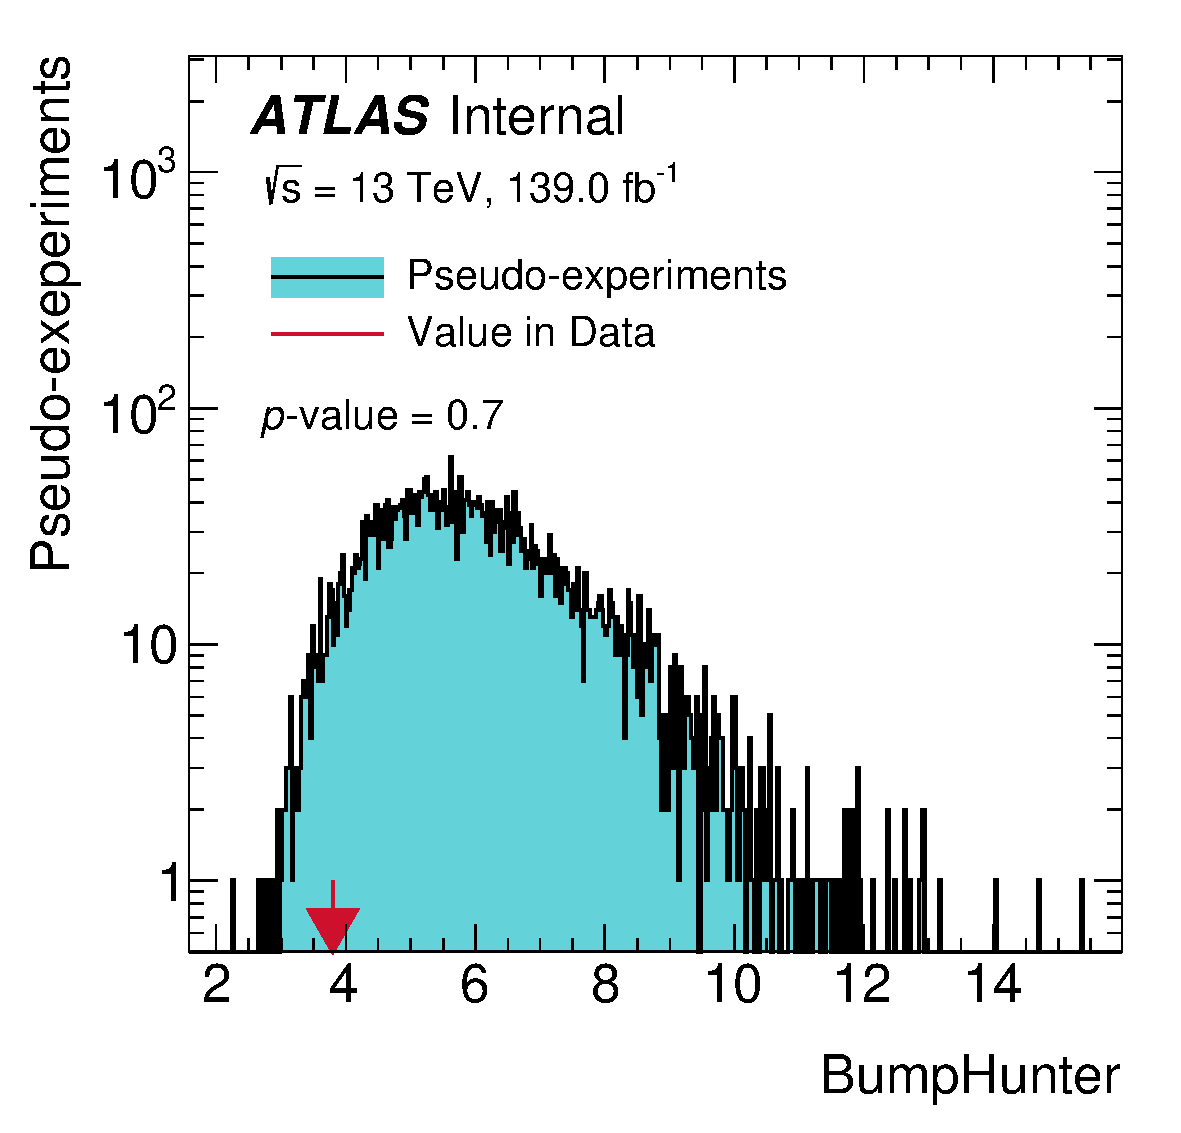
\includegraphics[width=0.30\textwidth]{figures/chapter_dimuon/bumpHunterStatPlot}        
        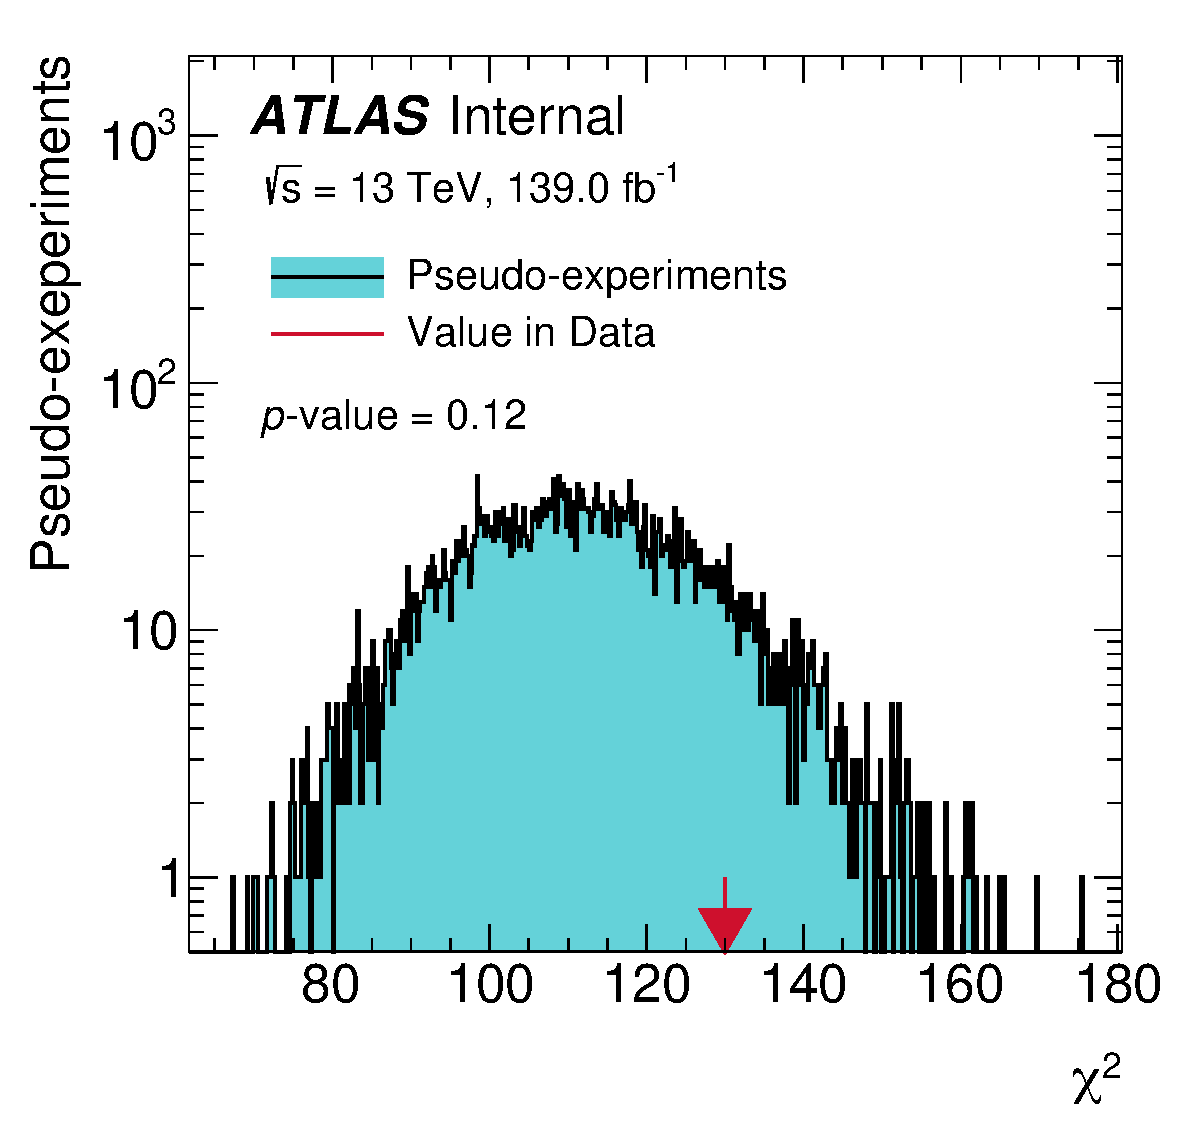
\includegraphics[width=0.30\textwidth]{figures/chapter_dimuon/chi2StatPlot}        
        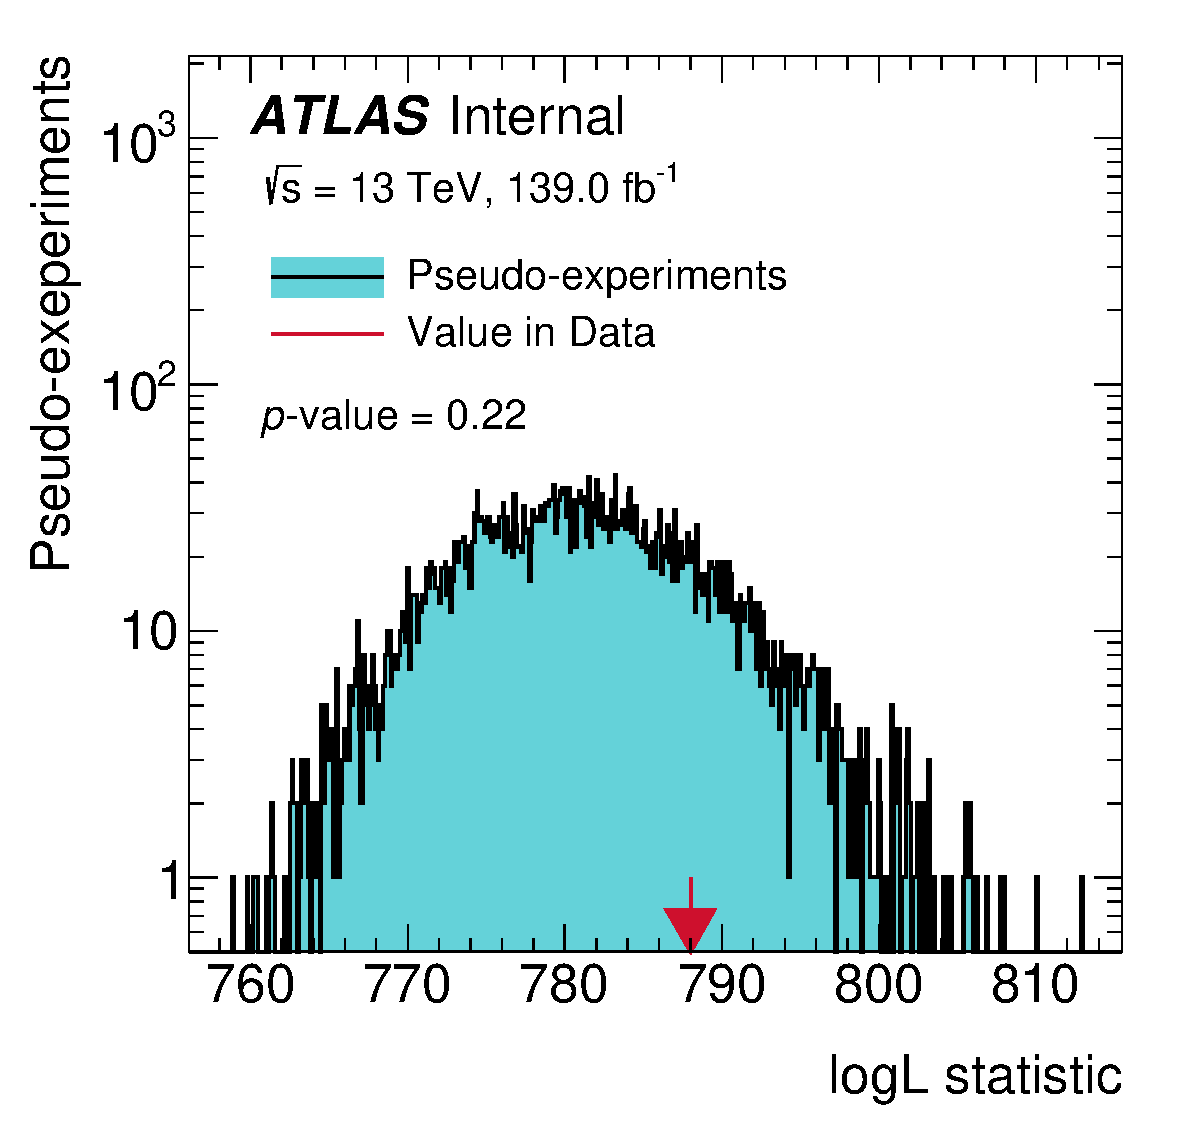
\includegraphics[width=0.30\textwidth]{figures/chapter_dimuon/logLStatPlot}        
        \caption{
        These plots illustrates the test statistics of the nominal fit compared against the pseudoexperiment test statistics distribution. }
        \label{fig:nominalstats}
    \end{center}
\end{figure}
\FloatBarrier


\subsection{Hyperparameter Optimization}
The detailed steps to the hyper-parameter optimization can be found in Chapter~\ref{chapter:analysismethod} in Section~\ref{sec:hyperparam}.
The lower bound on the lengthscale of the background kernel and the signal kernel are finalized from the signal injection test result in Section~\ref{sec:signalinjection} and Section~\ref{sec:binnning} respectively. The other hyper-parameter are allow to float and is optimized for each fit performed. 

In the dimuon analysis, the background kernel fits are performed on different variation of the fast simulation MC to ensure the selected hyper-parameters and lengthscale are flexible enough for the variation possibly present in the final data. Figure~\ref{fig:dimuonmass} shows fitting result in the inclusive region of the MC using the background kernel listed in ~\ref{sec:fastsimulation}. The result shows that the lengthscale lowerbound chosen is flexible enough against changes in the distribution fluctuation. 

% Insert pictures

\begin{figure}[!htb]
    \begin{center}
        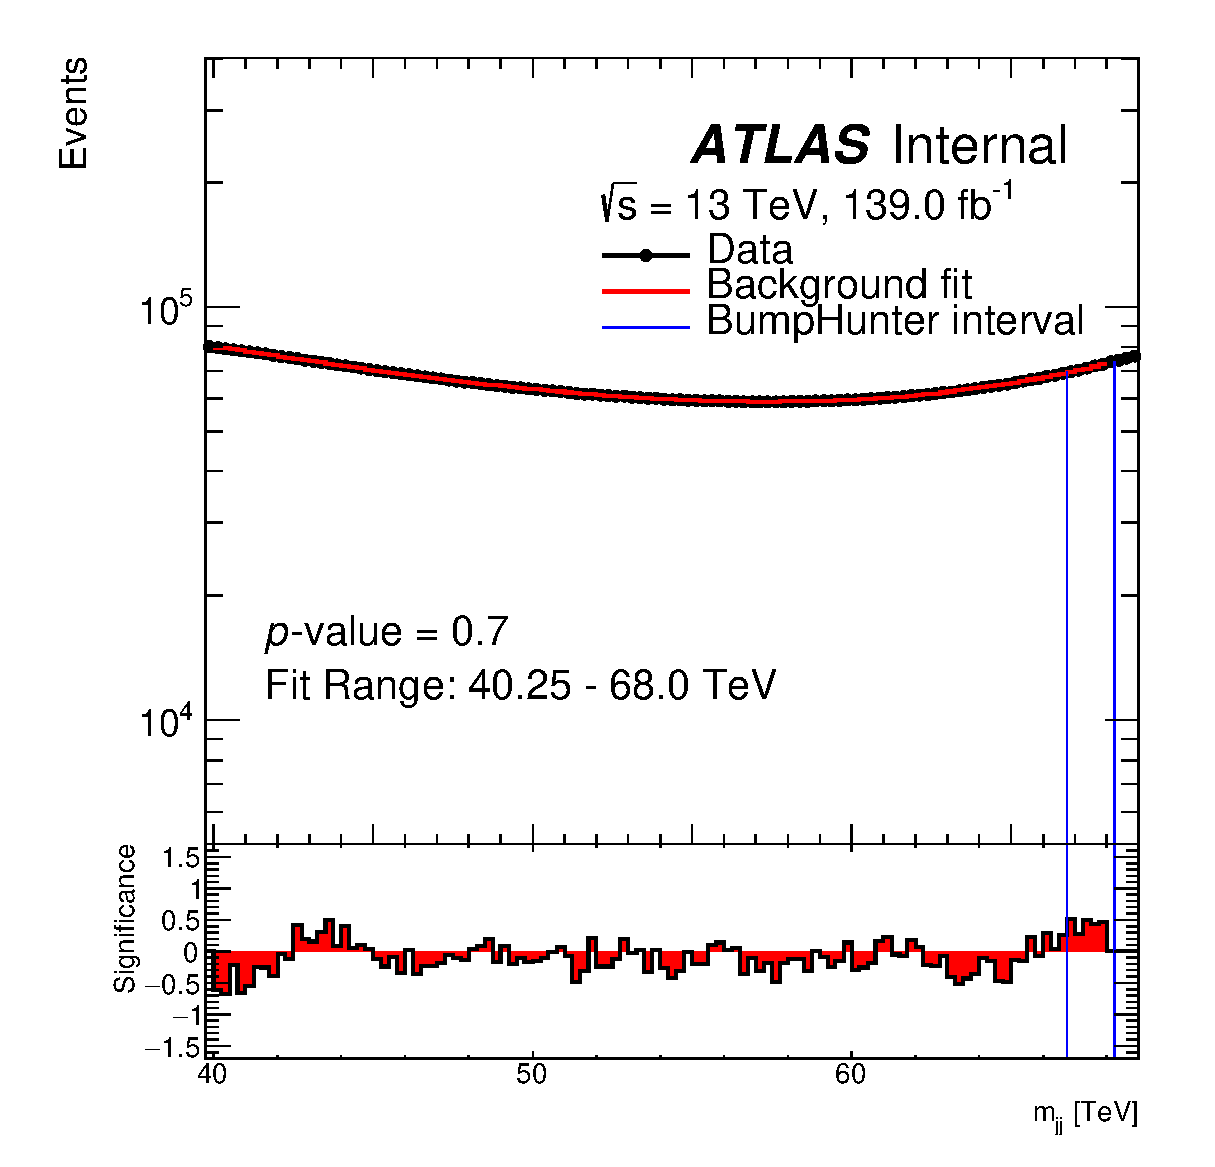
\includegraphics[width=0.45\textwidth]{figures/chapter_dimuon/nominal}        
        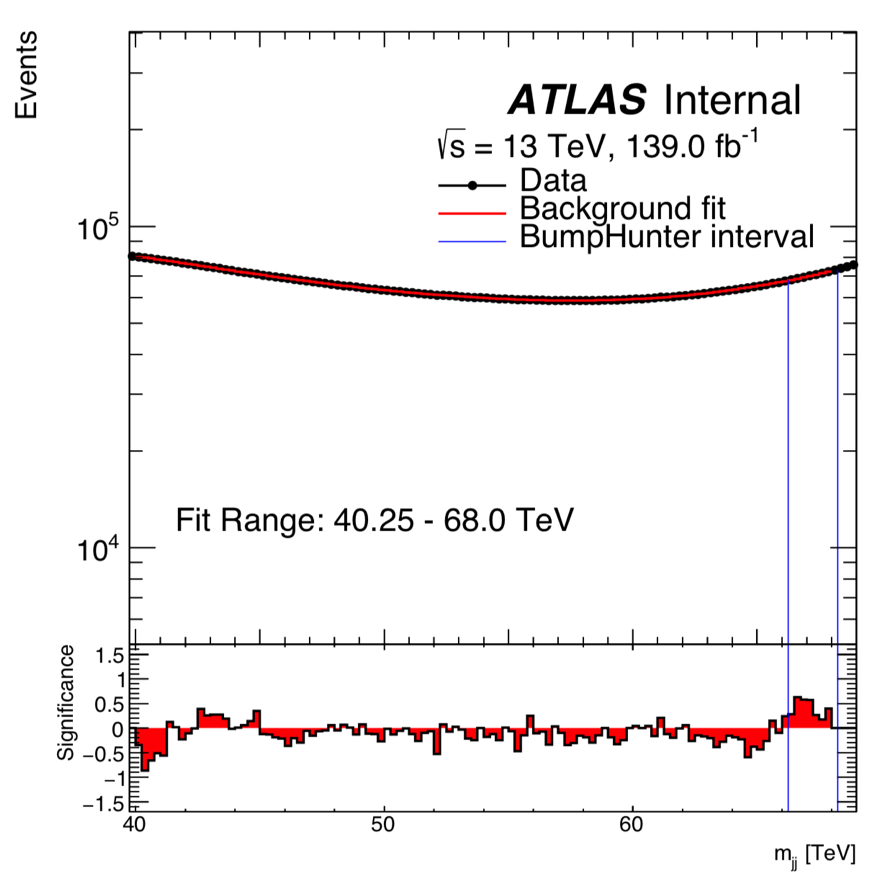
\includegraphics[width=0.45\textwidth]{figures/chapter_dimuon/up}        
        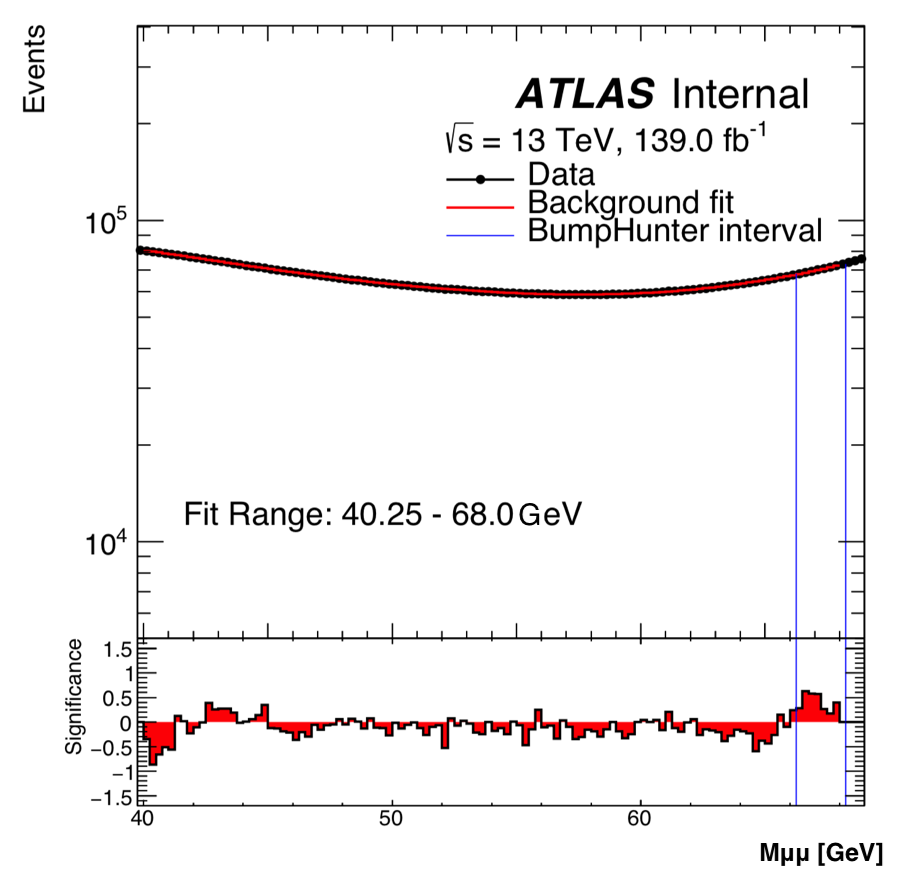
\includegraphics[width=0.45\textwidth]{figures/chapter_dimuon/down}        
        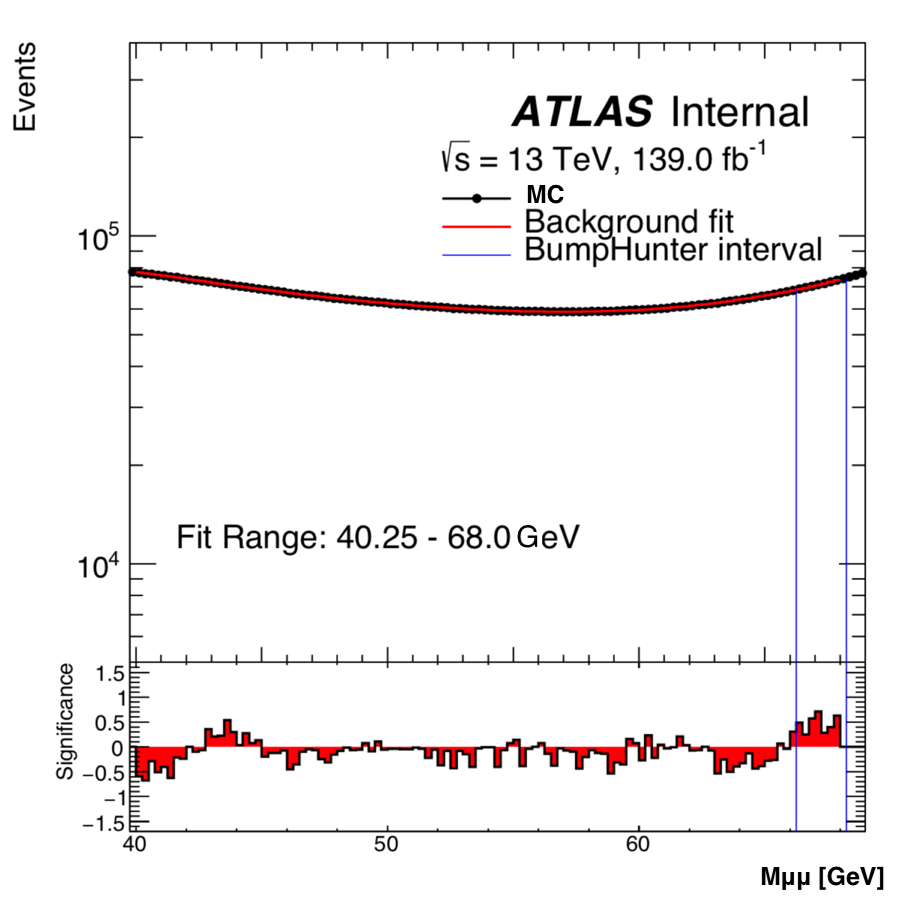
\includegraphics[width=0.45\textwidth]{figures/chapter_dimuon/eta}        
        \caption{
        These figures illustrates the Gaussian process background kernel fit on the different variation of fast simulation detailed in Section~\ref{sec:fastsimulation}. The fit test statistics as well as the residual in the bottom panel shows that the background kernel is able to capture features in the background variation. 
        }
        \label{fig:dimuonmass}
    \end{center}
\end{figure}
\FloatBarrier

\subsection{Background and Signal Estimation}
Studies found that the background estimation from the background kernel alone was not able to separate the background from the signal to a high efficiency, the final background and signal estimation are done through the following separation equations. Figure~\ref{fig:signalseparation} shows an example separation done by the method.

\begin{itemize}
    \item \textbf{Background Prediction}
    \begin{equation}
        \mu_{bkg}(x_{*}|y) = \mu_{\textrm{bkg kernel}}(x_{*}|y)+K_{\textrm{bkg kernel}}(x_{*}, x) \cdot K_{\textrm{sig+bkg kernel}}(x,x') \cdot( y(x)-\mu_{\textrm{bkg kernel}}(x_{*}|y) )
    \end{equation}


    \item \textbf{Signal Prediction}
    \begin{equation}
        \mu_{sig}(x_{*}|y) = K_{\textrm{sig kernel}}(x_{*}, x)\cdot K_{\textrm{sig+bkg kernel}}(x,x') \cdot ( y(x)-\mu_{\textrm{bkg kernel}}(x_{*}|y) )
    \end{equation}

\end{itemize}

\begin{figure}[!htb]
    \begin{center}
        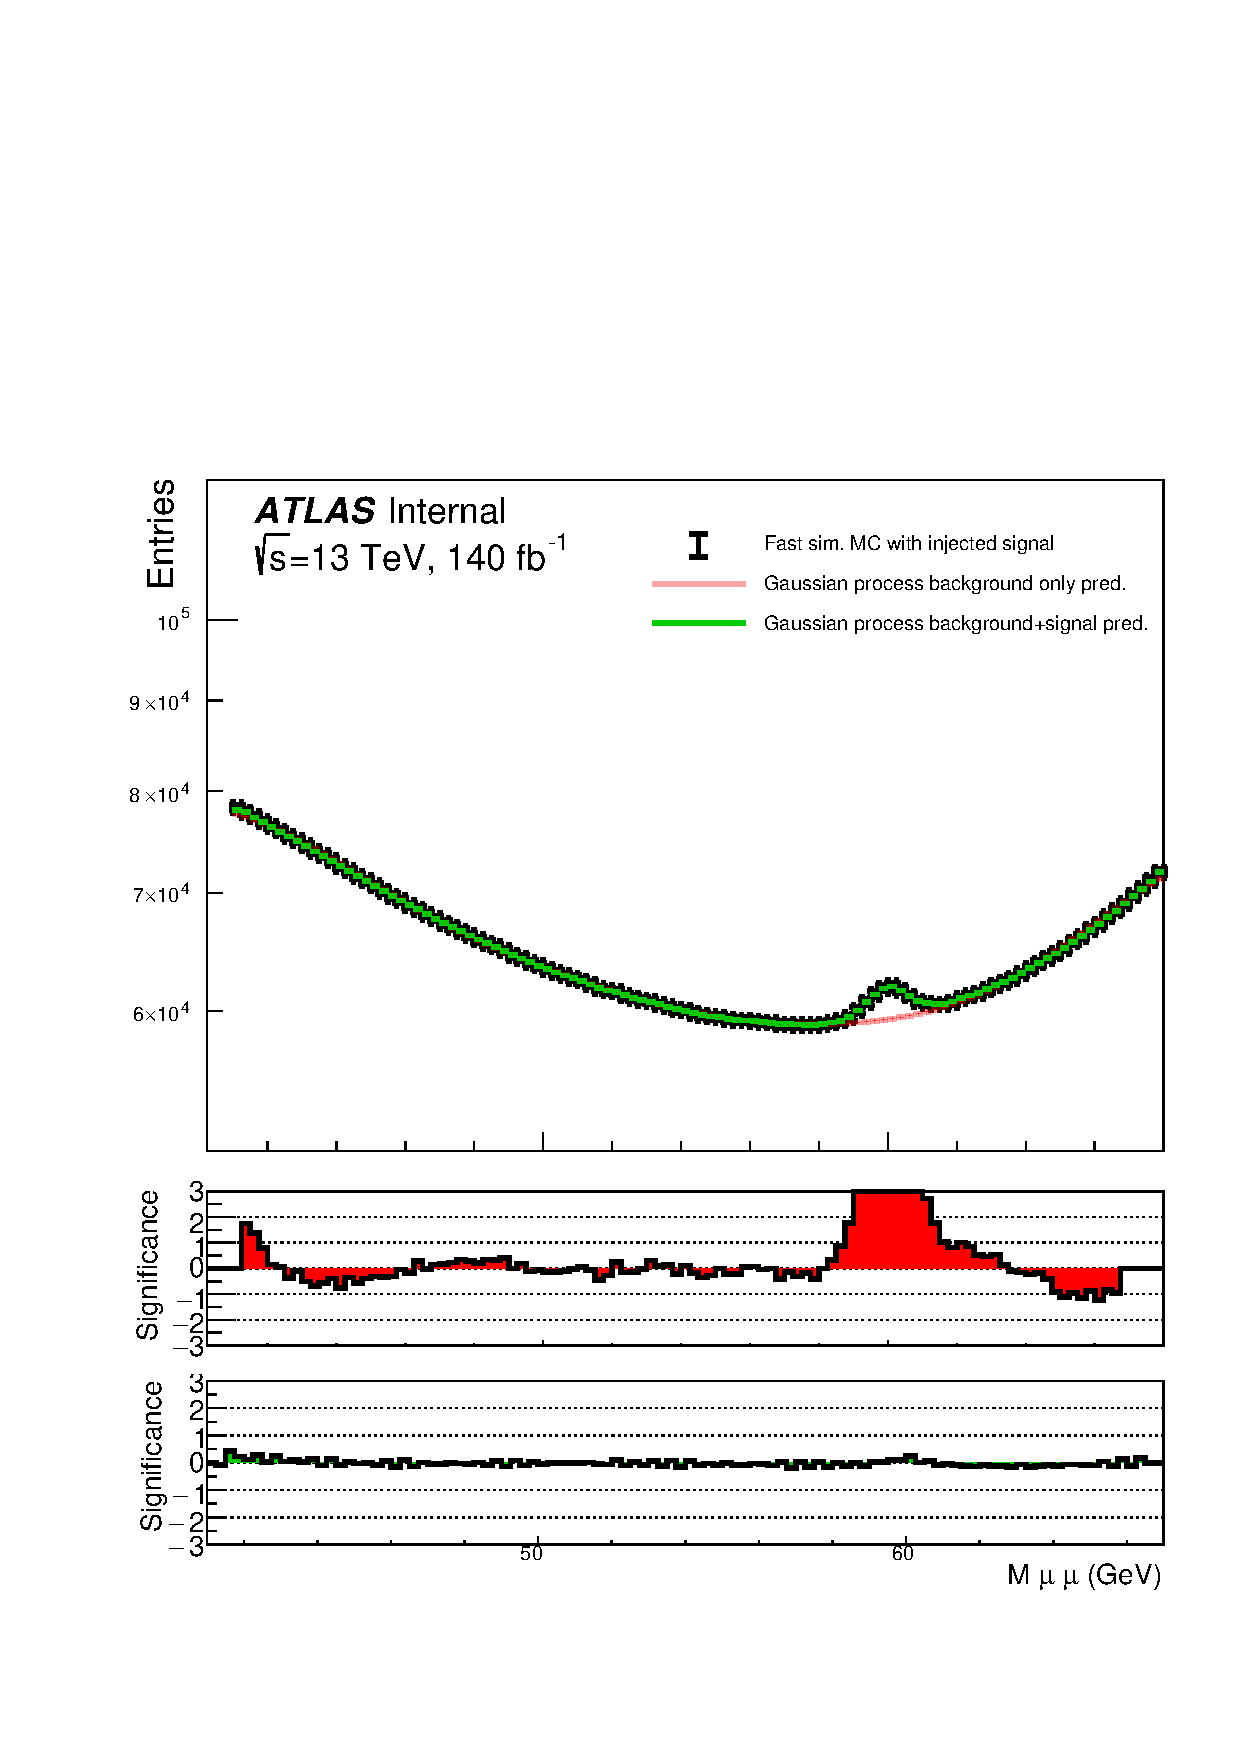
\includegraphics[width=0.45\textwidth]{figures/chapter_dimuon//BackgroundSeparated}        
        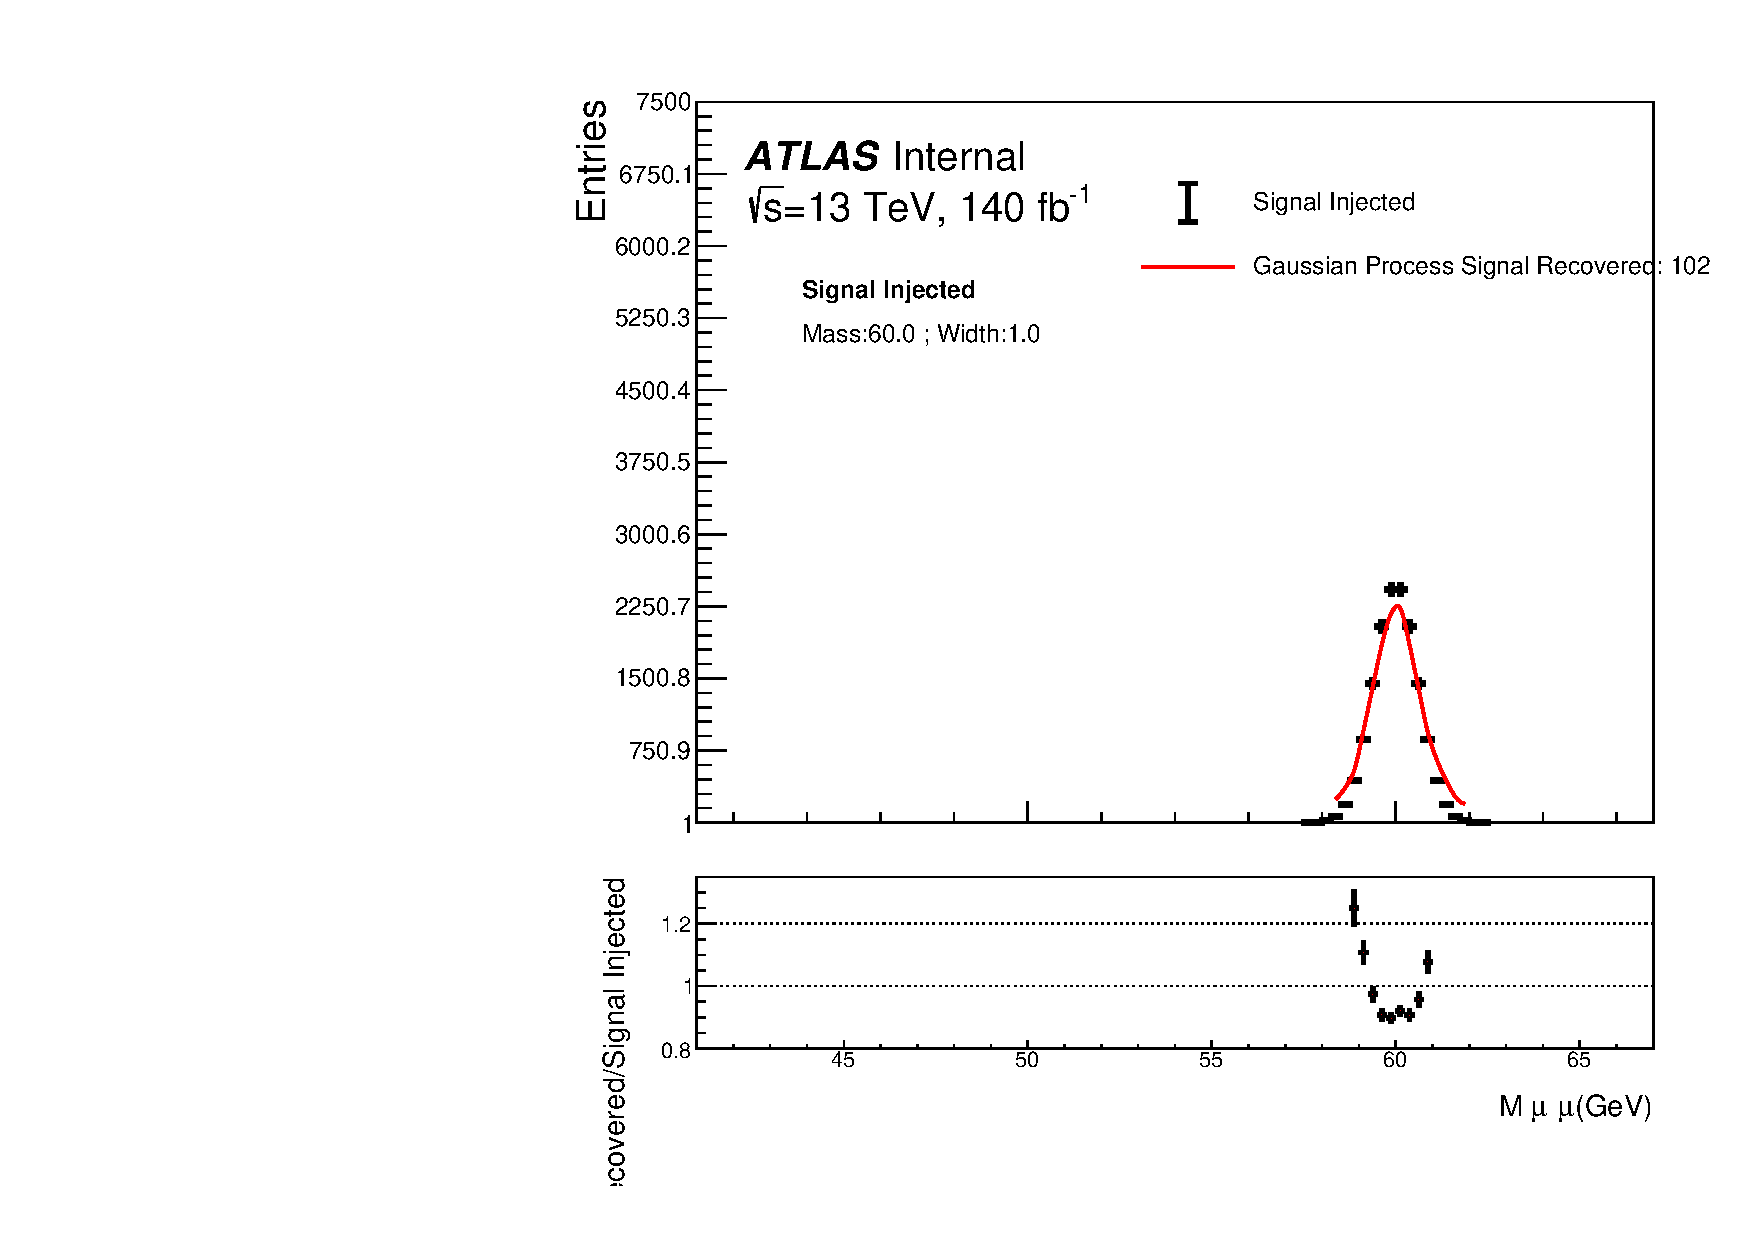
\includegraphics[width=0.45\textwidth]{figures/chapter_dimuon/SignalSeparated}        
        \caption{
            These figures illustrates the background and the signal separated from the signal injected background MC. The signal reconstruction yield for this particular signal is up to 94\%.
        }
        \label{fig:dimuonmass}
    \end{center}
\end{figure}
\FloatBarrier


\subsection{Background Prediction Performance Studies}
The Gaussian Process background prediction went through testing suggested in the ATLAS smoothing recommendation document to ensure the smooth background procedure is valid for resonance searches. Two tests, the signal injection test and the spurious signal test are conducted to ensure the background estimation is sensitive to signal above a certain size and the background error is within acceptable range of the estimation. The following subsection shows the results using background prediction on ATLAS background MC.  

\subsubsection{Signal injection test} 

%\textit{-``Test for smallest signal the background estimation is sensitive to”}

This section detailed the procedure to the signal injection test Section~\ref{sec:signalinjection}. Only results are presented here.

It\'s found that a minimum lengthscale of 4 GeV is needed for the background kernel for the background model to be sensitive to signal of 3 $\sigma$ background error size and above in the 45-68 GeV range in the inclusive region. Most of the signal width used passed the test when this lengthscale is chosen. 

\begin{figure}[!htb]
    \begin{center}
        \includegraphics[width=0.75\textwidth]{figures/chapter_dimuon/signalInjection}        
        \caption{
        This figure illustrate a signal injection test performed at the mass point 55GeV of 3\% mass width. In the first panael, the red line shows the background MC + signal injected divided by the background MC; the green and the red line is the fit ratio of the "just above" triggering background fit against the background MC and the "just below" trigger of the bumphunter fit against the background MC. The grey bands shows the width of the background error. Results shows that the the fit is sensitive to signal $<$ 3 $\sigma$ of the background error in this mass point and width. }
    \label{fig:dimuonstudies}
    \end{center}
\end{figure}
\FloatBarrier

\subsubsection{Background Modelling}
Using the minimal lengthscale chosen for the background and allowing other hyperparameters to float, tests fits are performed on the nominal fit, and also done on the different statistical variation of the background, the 1 $\sigma$ up and 1 $\sigma$ down variation of the fast simulation Pythia, as well as the $\eta$ variation, defined in Section~\ref{sec:fastsimulation}.
The fitting result shows that lengthscale chosen for Gaussian Process works well for all of these statistical variations. 

\begin{figure}[!htb]
    \begin{center}
        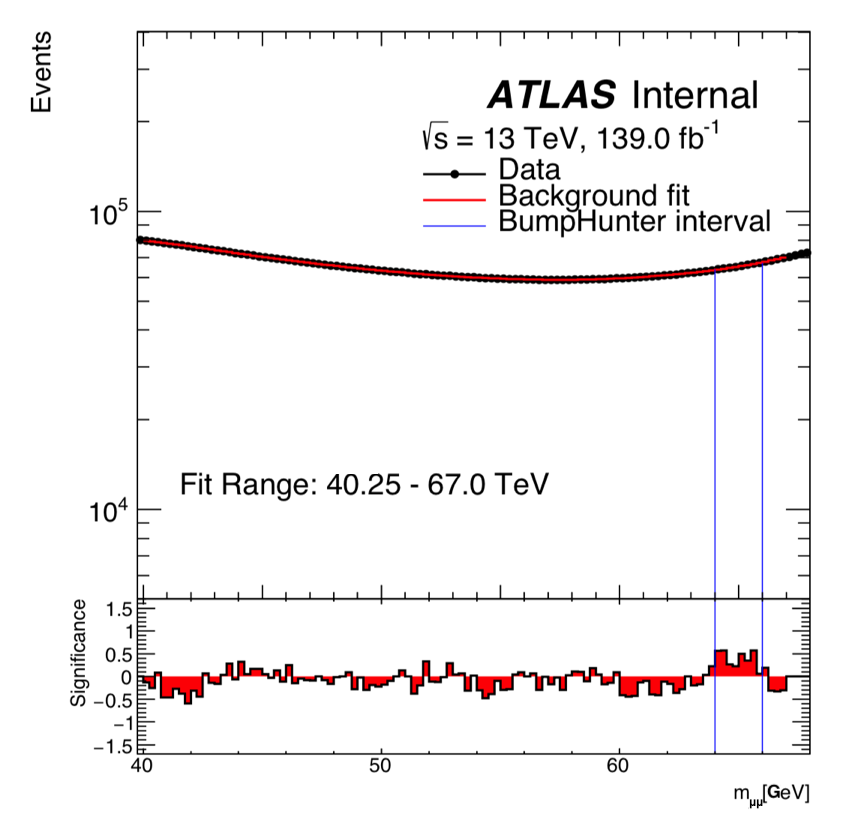
\includegraphics[width=0.45\textwidth]{figures/chapter_dimuon/Nominal}        
        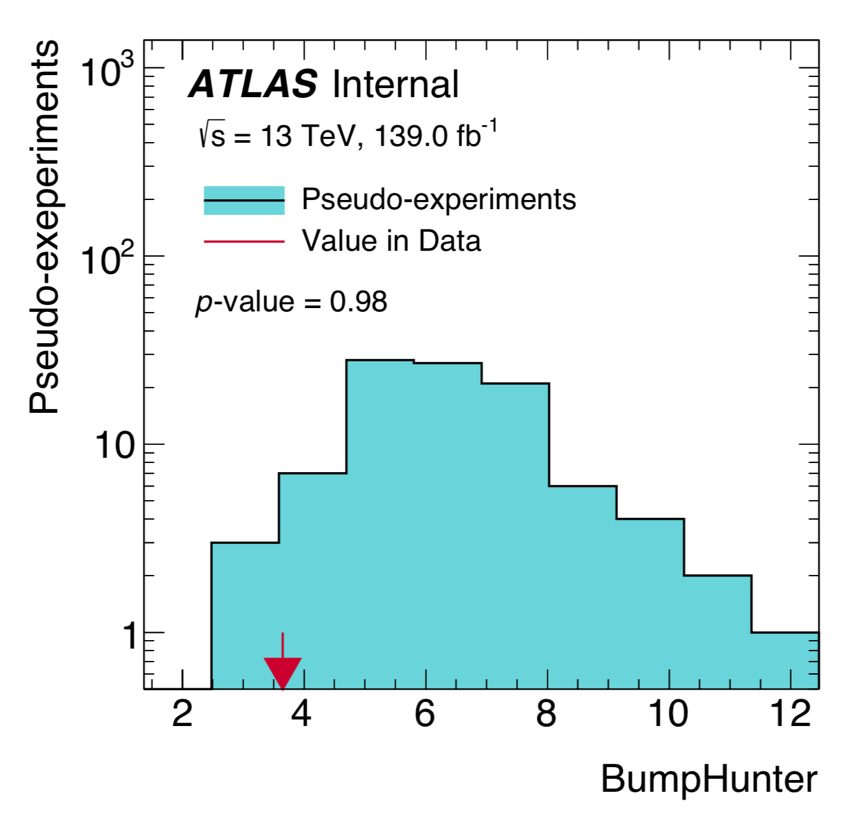
\includegraphics[width=0.45\textwidth]{figures/chapter_dimuon/NominalBH}        
        %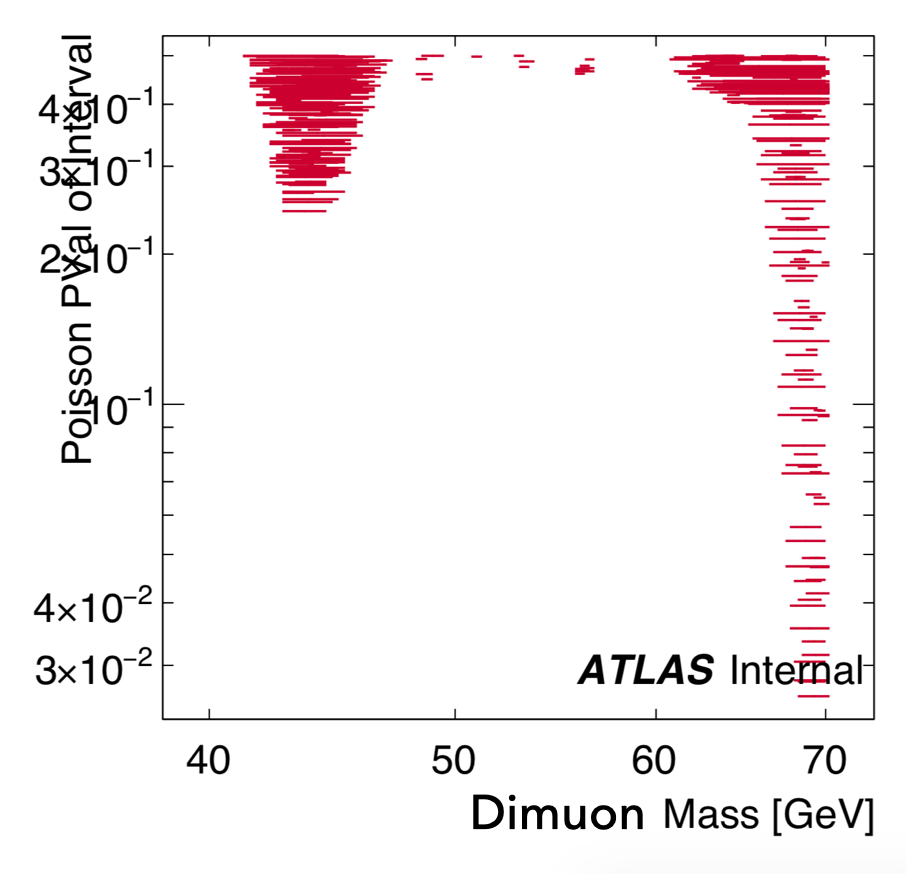
\includegraphics[width=0.30\textwidth]{figures/chapter_dimuon/NominalFit}        
        \caption{
        These figure illustrates the nominal fit, along with the bumphunter test statistics and the observed value distribution. It is shown that the most discrepant window does not fall below the critical p-value of 0.01. Details on the bumphunting procedure can be found here. 
        }
        \label{fig:dimuonstudies}
    \end{center}
\end{figure}
\FloatBarrier



\subsection{Spurious signal test}

The spurious signal test is a test that defines the uncertainty relative to signal yield. Details are presented here in Section~\ref{sec:spurious}.
The spurious signal test is considered passed if the signal extracted versus background error ratio is $<$ 0.5.
The spurious signal test results on the Gaussian process is shown in Figure~\ref{fig:spurious}:
Currently ongoing work on is being done to further reduce the spurious signal.

\begin{figure}[!htb]
    \begin{center}
        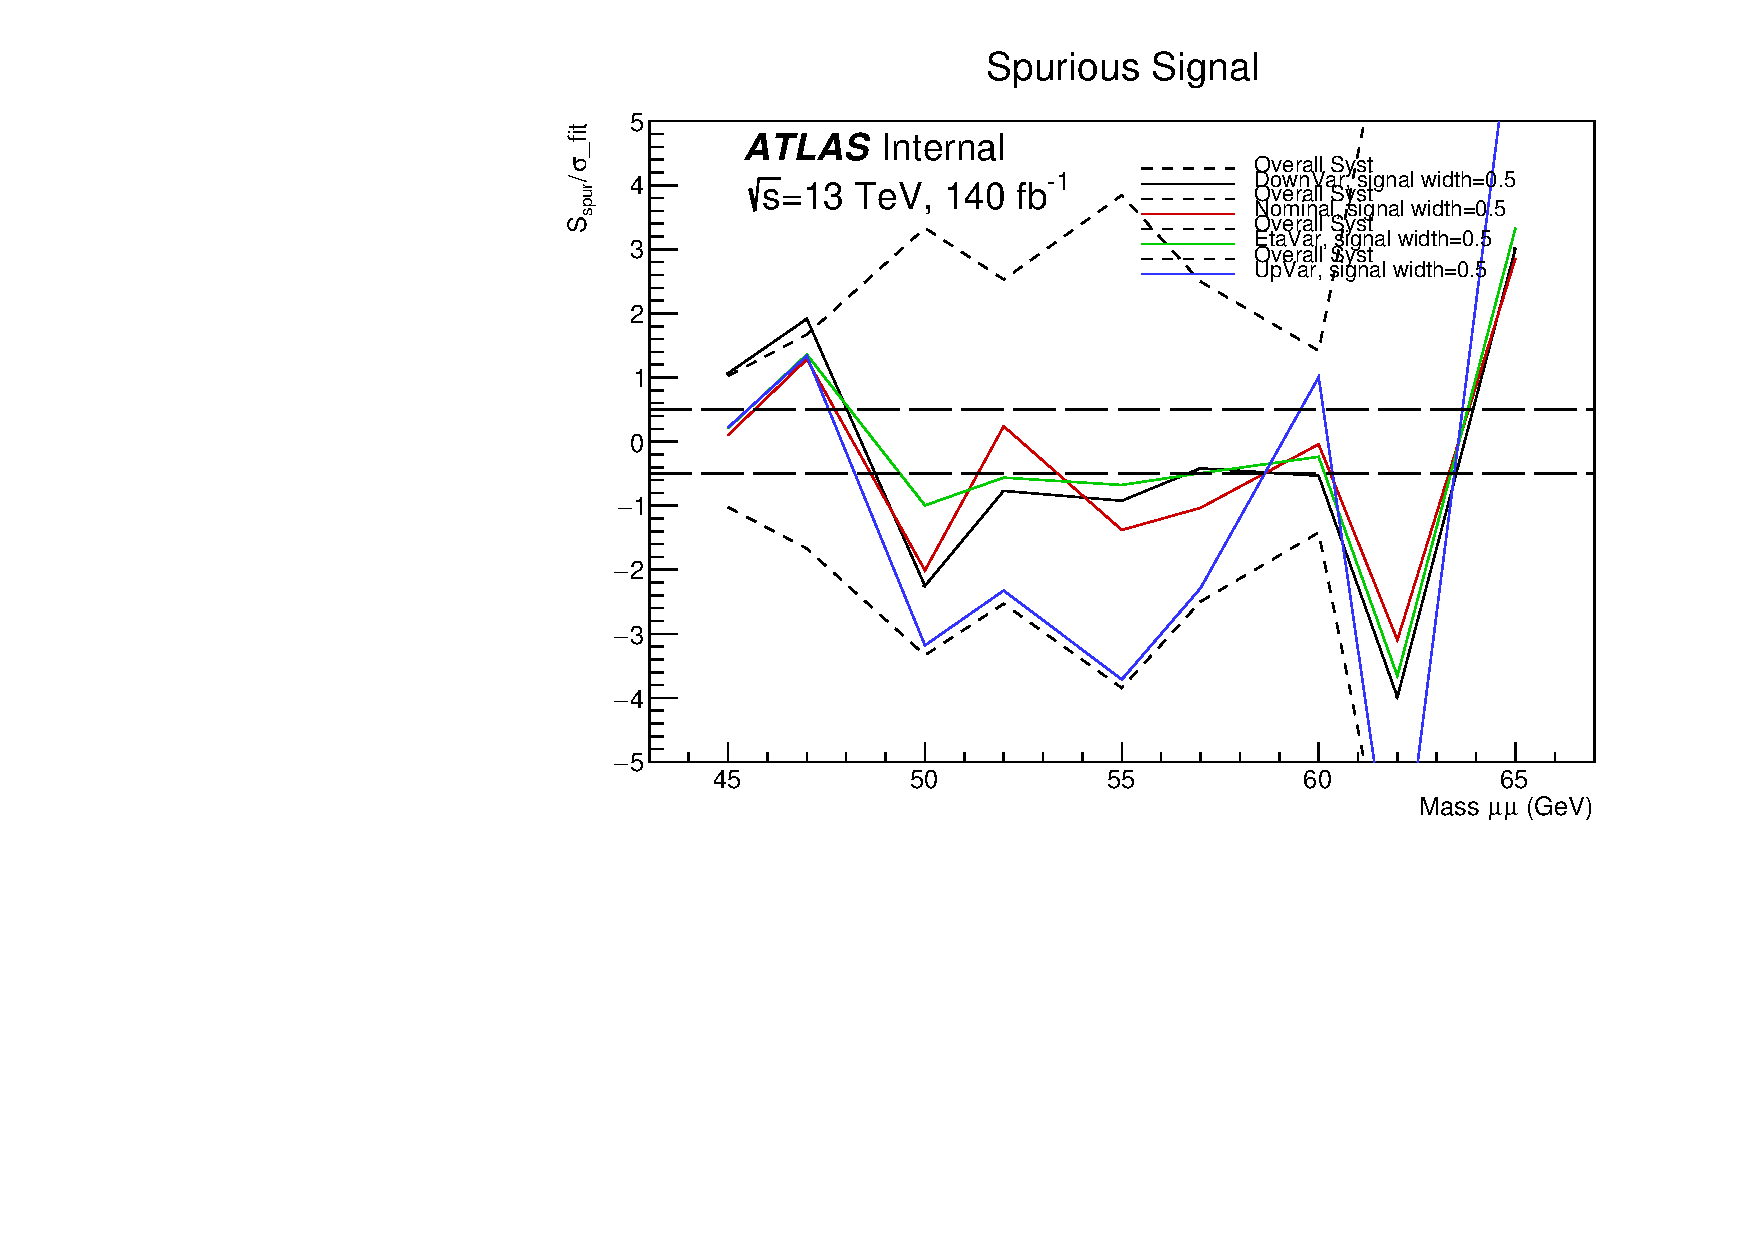
\includegraphics[width=0.75\textwidth]{figures/chapter_dimuon/spurious}        
        \caption{
        This figure illustrate a spurious signal test result on the different background variation fits.}
        \label{fig:spurious}
    \end{center}
\end{figure}
\FloatBarrier

\section{Statistics Testing}
Details on the statistical test can be found here~\ref{section:stats}. During the time where the thesis was written, the data was not unblinded. Monte Carlo studies were done to verfied the procedure. The following statistical tests has been presented in the CERN Statistical Forum.

\section{The Search}

\textit{``The Rejection/Acceptance of the null hypothesis"}

The search aims to either accept or reject the null hypothesis. Details are listed in this Section~\ref{sec:thesearch}.

An example of the search done with just the background and no signal injected is shown in Figure~\ref{}. The test statistics, including 
the loglikelihood, the $\chi^{2}$ and the bumphunter test statistics all have p-value below 0.01. No anomaly is found and the null hypothesis is accepted.
    
\begin{figure}[!htb]
    \begin{center}
        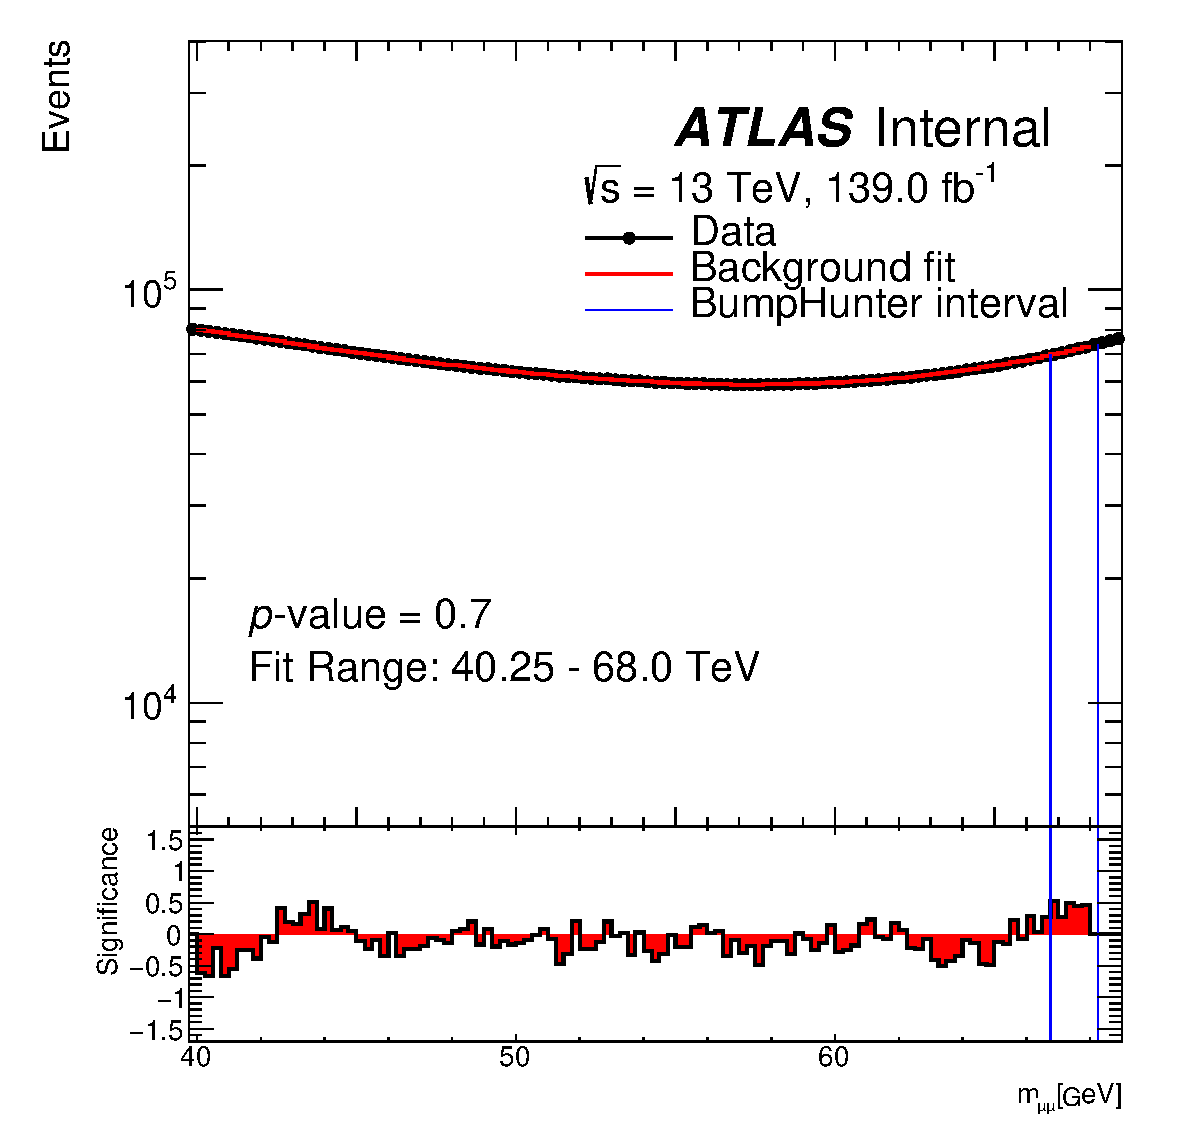
\includegraphics[width=0.45\textwidth]{figures/chapter_dimuon/nominal_fixed}
        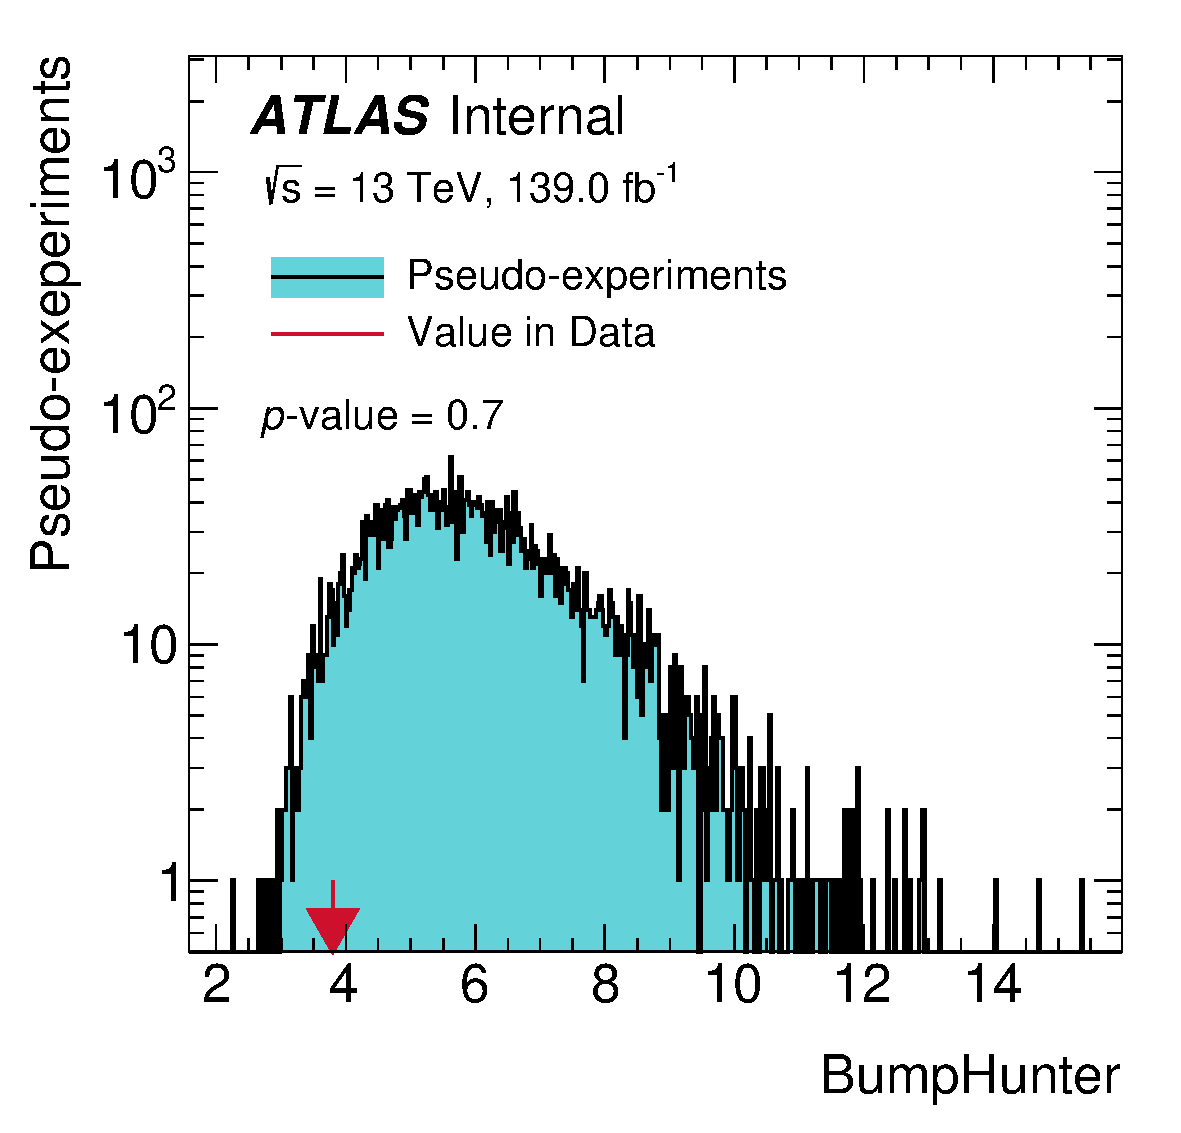
\includegraphics[width=0.45\textwidth]{figures/chapter_dimuon/bumpHunterStatPlot}
        \caption{
        These figures illustrate a statistical test on background only MC, the p-value is observed to be way above the 0.01 cut off for anomaly. In  this case the null hypothesis is accepted.
        }
    \label{fig:dimuonstudies}
    \end{center}
\end{figure}
\FloatBarrier

An other example of the search done with the background plus signal injected in 50 GeV. The bumphunter test statistics have p-value below 0.01. The null hypothesis is rejected. In this scenario, there could be Beyond-the-Standard-Model signal present in the data.

\begin{figure}[!htb]
    \begin{center}
        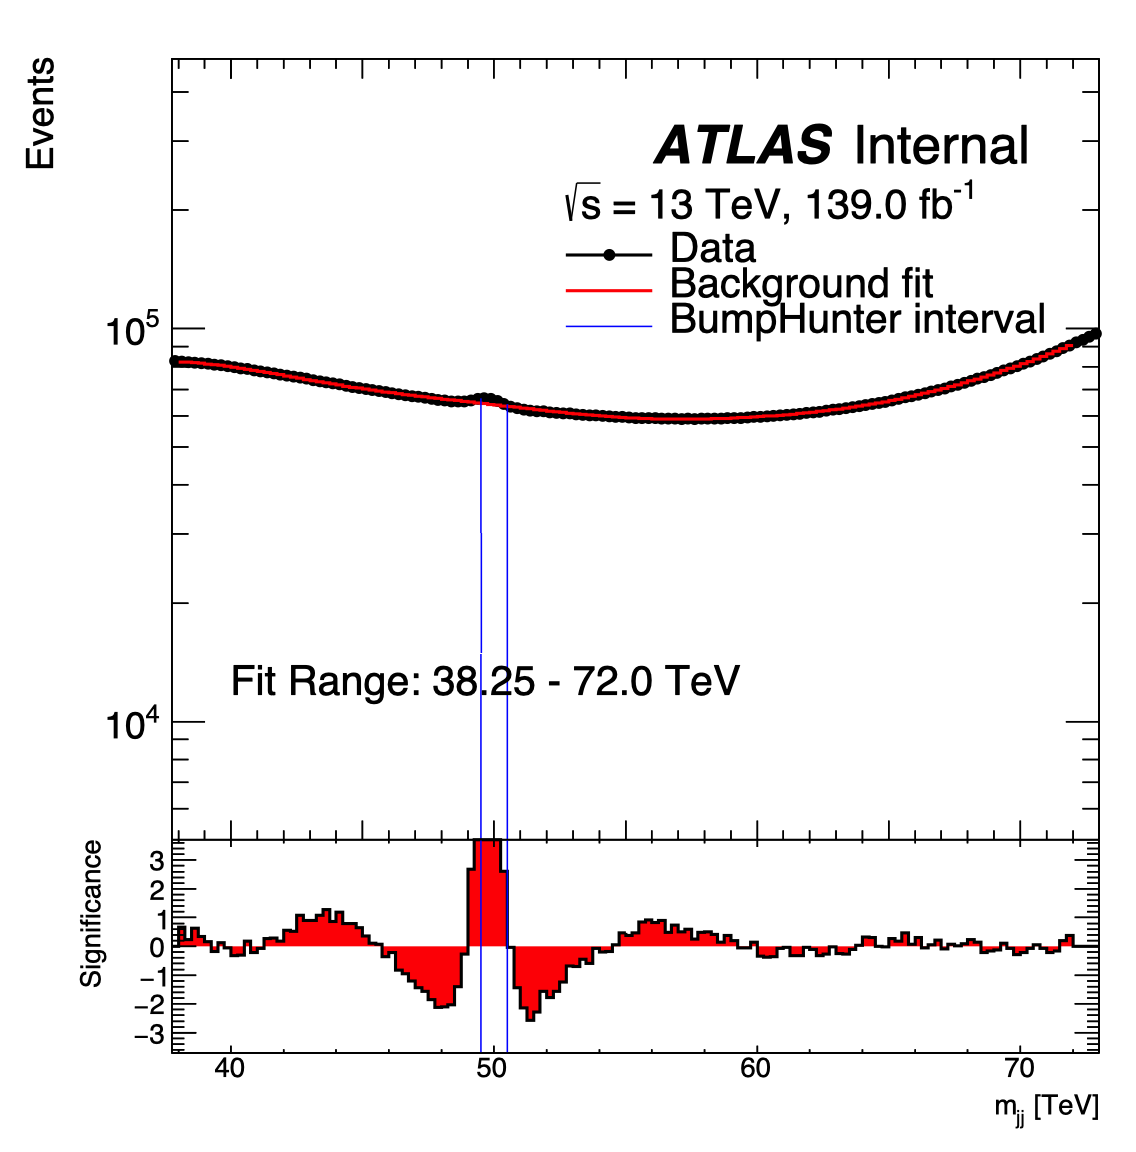
\includegraphics[width=0.45\textwidth]{figures/chapter_dimuon/SearchBump}
        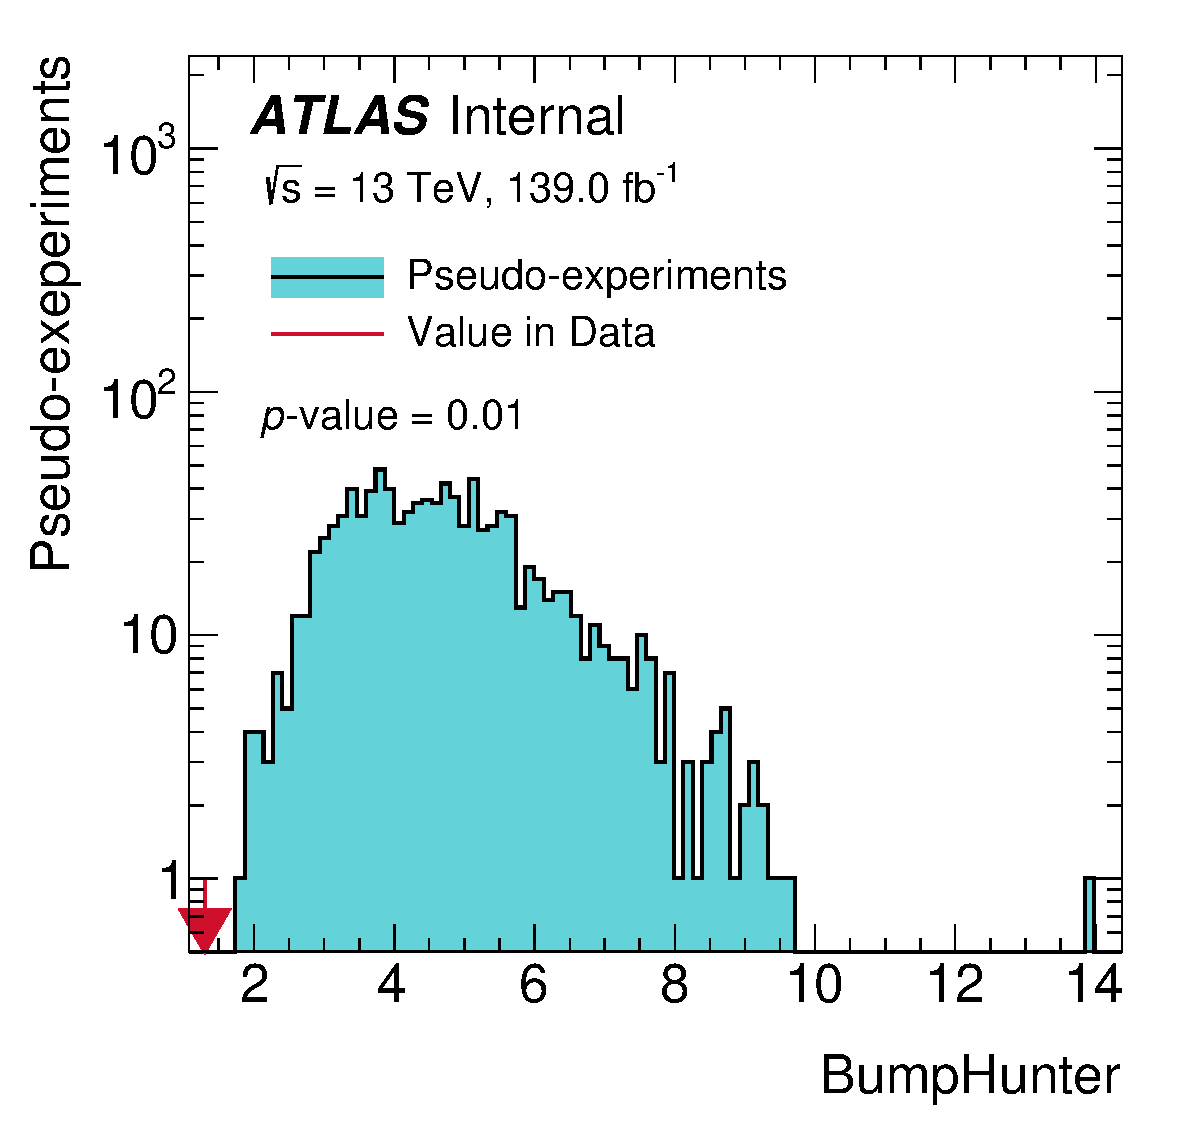
\includegraphics[width=0.45\textwidth]{figures/chapter_dimuon/bumpHunterStatPlot_bump}
        \caption{
        These figures illustrate a test done on signal injected at 55 GeV, and the window exclusion that picked out the signal injected in there.}
%            \label{fig:dimuonstudies}
    \end{center}
\end{figure}
\FloatBarrier

The results shows that the statistic test of the search is in place for when the data is ready to be unblinded.

\section{Limit Setting}

\textit{``Finding signal strength value where the alternative hypothesis is rejected to a 95\% confidence level"}

The limit setting aims to find the upper limit for the signal strength at 95\% confidence level. In the dimuon analysis, the limit setting procedure is done through the Asimov approximation of the frequentist limits described in ~\ref{sec:limits}.

Preliminary limit setting based on Gaussian Process is still currently under test. In alternative fit function limits calculated by approximation based on the fit function method is shown here in Figure~\ref{fig:limits}.

\begin{figure}[!htb]
   \begin{center}
       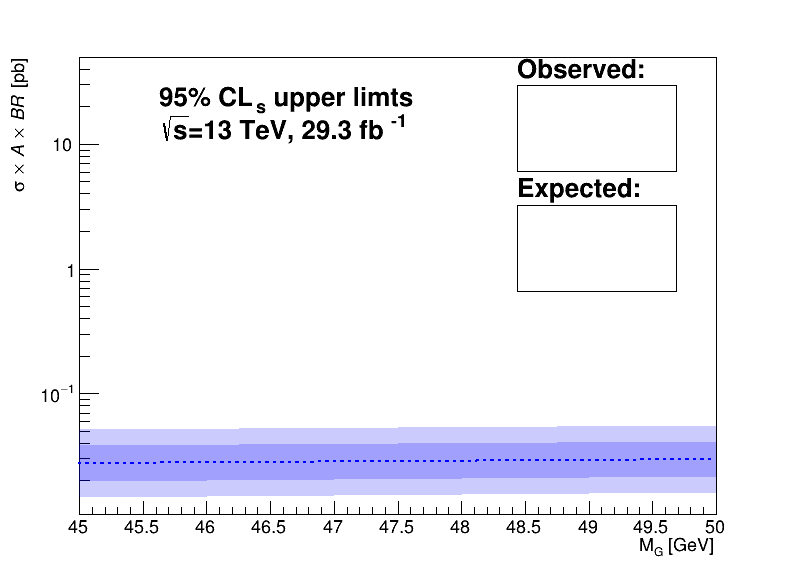
\includegraphics[width=0.75\textwidth]{figures/chapter_dimuon/limits}
       \caption{
       This figure illustrate a spurious signal test result on the different background variation fits.}
        \label{fig:limits}
   \end{center}
\end{figure}
\FloatBarrier

\section{Future Work}
The analysis is on its way to completing the final strategies and to be unblinded on data soon.

%Adding the Gaussian process limit to the background

%\section{Alternative fitting}
%An alternative fitting method is done through the fit function method.

%\section{Systematics}
%section{Future Extensions}

